\documentclass[11pt]{article}
\usepackage[left=20mm, right=20mm, top=20mm, bottom=20mm]{geometry} %this sets the page margins 
\usepackage[backend=bibtex]{biblatex}
\addbibresource{references.bib}
\usepackage{amsmath}
\usepackage{amsfonts}
\usepackage{amssymb}
\usepackage{graphicx}
\usepackage{wrapfig}
\usepackage{subcaption}
\usepackage[justification=centering]{caption}
\usepackage{setspace}
\doublespacing
\setlength{\parindent}{1cm}
\usepackage{color}
\usepackage{framed}
\usepackage{comment}
\usepackage{pdfpages}
\usepackage{courier}
\usepackage{float}
\usepackage{helvet}
\renewcommand{\familydefault}{\sfdefault}
\usepackage{listings,xcolor}
\usepackage[numbered,framed]{matlab-prettifier}
\renewcommand{\lstlistingname}{Codebox}% Listing -> Codebox
\usepackage{breqn}
\usepackage{mathtools}


\newcommand\undermat[2]{%
  \makebox[0pt][l]{$\smash{\underbrace{\phantom{%
    \begin{matrix}#2\end{matrix}}}_{\text{$#1$}}}$}#2}

\numberwithin{equation}{subsection}
\usepackage{titlesec}
\newcommand{\sectionbreak}{\clearpage}
\DeclareMathOperator\arctanh{arctanh}
\DeclareMathOperator\erf{erf}

%% THIS BIT MAKES CLICKABLE PDF LINKS
\usepackage{hyperref}
\hypersetup{
    colorlinks,
    citecolor=black,
    filecolor=black,
    linkcolor=black,
    urlcolor=black
}
%%


\author{Henry Fletcher}

\title{Making Flash Memory Work}

%%%%%%%%%%%%%%%%%%%%%%%%%%%%%%%%%%%%%%%%%%%%%%%%%%%%%%%%%%%%%%%%%%%%%%%%%%%%
\begin{document}

\section{Executive Summary}

Modern flash memory is reliant on error-correcting code to ensure error-free operation. Current flash memory architectures often use linear block codes for this purpose (e.g. Reed-Solomon, Hamming or BCH codes). However, the recent rediscovery of LDPC (Low Density Parity Check) codes, which can achieve superior performance close to the Shannon Limit, has generated much interest in the NAND memory industry. These codes could be used to further improve error correction capability in flash memory, thus allowing for more densely packed memory cells and thus larger capacity drives.

The general aim of this project is to produce a MATLAB simulation of how an error correction system using LDPC codes would work for flash memory.  By combining both an error generation and an error correction model, it will be possible to benchmark these rediscovered codes, and subsequently compare them to current generation technologies.

\tableofcontents

\section{Introduction}
[Disclaimer: Intro needs further work!] Flash Memory is a multi-billion dollar industry, and is almost certainly set to grow in the future. It is also a highly competitive one, with consumers eager for low cost yet high volume storage. Innovation in the industry therefore seeks to increase the capacity and performance of these drives whilst keeping manufacturing costs low. 

An obvious way to achieve low cost per Gigabyte is to increase the number of stored bits per cell without increasing the number of physical memory cells. Indeed, most consumer high capacity solid-state drives use this approach, making use of MLC (Multi-level cell) or TLC technology where 2 or 3 bits of information are stored per cell. However this comes at the cost of reducing read/write speeds, as well as increasing the occurrence of bit-errors on the device. 

Current generation flash memory therefore makes extensive use of Error-Correcting Code, to offset the increased error rate caused by densely packed cells. However, recent advances in error-correction capability elsewhere have yet to be implemented in consumer flash memory devices. This project therefore aims to investigate the use of the latest generation error-correcting codes in flash memory. 

Previous papers [??,??,??] on this topic have investigated the use of more modern error-correcting codes, including a type known as Low Density Parity Check (LDPC) codes, and have shown performance improvements over existing coding schemes. In addition, these papers present a more accurate noise model for flash memory, that takes into account the program/erase nature of the memory cells. Previous work on LDPC codes is extensive [??,??,??], particularly by MacKay who rediscovered them. The decoding method for these codes, the Belief Propagation algorithm, also features in a large number of papers [??........], and in addition methods for simplifying this decoding method through the use of approximations [??,??,??].

The majority of this project concerns the development of a MATLAB simulation, that includes both an error generation and error correction model. The flash memory error model, used to simulate the effects of noise and time-varying degradation in a memory cell, is mostly derived from existing work. So too are the methods for error correction, in the form of LDPC and the Belief Propagation algorithm. However, the novelty of this project is investigating how varying degrees of prior information provided to the decoder can alter error performance, through using approximations of the underlying noise assumptions. It also seeks to show the importance of modelling the noise correctly, since having an accurate noise model will result in superior system performance.

\section{Overview of Linear Block Codes}

Linear block codes are one of the two main classes of forward error correction (FEC), with the other main type being convolutional coding. A linear block code essentially takes a block of binary data, and adds additional redundant data onto it. This block can then be transmitted over a noisy channel, and subsequently decoded at the receiver. The redundant bits in the block are used as parity check equations, which allows a linear block code to both detect and correct errors. 

\subsection{Definitions for Linear Block Codes} \label{3.1:definitions}
All linear block codes can be described using a set of standard terms and symbols. For this project, all codes use a binary alphabet of $\{0,1\}$ and hence all operations are over this binary field. $n$ is the block length, the total size of the output codeword. $k$ is the message length, the size of the information vector prior to encoding. An $(n,k)$ error correcting \textit{code} $\mathcal{C}$, will produce a set of $2^k$ output \textit{codewords} $\mathbf{c}$. Hence, $\mathbf{c} \in \mathcal{C}$. 

The rate of any linear block code, $R$, is defined as: 
\begin{equation}
R = \dfrac{k}{n}
\end{equation}
The rate is a measure of the number of information bits compared to the total number of transmitted codeword bits. A high rate code will be more efficient in terms of useful information transmitted, but will have a poorer error correction capability. In Flash Memory, very high rate ($R > 0.9$) codes are used in order to maximise the amount of usable storage space. Conversely, an example use of low rate codes would be in deep-space probe transmissions, where receiving error-free data is more important than rate of transmission.

A linear block code can be represented in two ways: through the $k \times n$ generator matrix $\mathbf{G}$, or the $(n - k) \times n$ parity check matrix $\mathbf{H}$. Each is the null-space of the other, such that:
\begin{equation}
\mathbf{G H}^\top = 0
\end{equation}
Unsurprisingly, the generator matrix $\mathbf{G}$ is used in the transmission side when encoding data, and the parity check matrix $\mathbf{H}$ is used at the receiver to detect and correct any errors.

At the transmitter, if we take a $1 \times k$ input vector of binary data $\mathbf{x}$, the method of encoding this data into a codeword $\mathbf{c}$, is simply a multiplication operation:
\begin{equation}
\mathbf{c = xG}
\end{equation}
At the receiver, a similar operation is performed:
%%%% CHECK THAT THIS IS CORRECT !!! %%%%%
\begin{equation}
\mathbf{s = c H}^\top
\end{equation}
where $\mathbf{s}$ is known as the \textit{syndrome}. If the syndrome is the all zero vector, then error free transmission has occurred. Conversely, if any bit of the syndrome is 1, then this represents a particular error pattern. For small block lengths, these error pattern's can be pre-calculated and saved as a table, allowing for syndrome lookup decoding. The table identifies the exact location of a bit error in the codeword, which can then be `flipped' in order to perform error correction.

An example of a \textit{systematic} generator matrix, in this case a matrix known as the \textit{Hamming(7,4) code}, takes the form:
\begin{equation}
\mathbf{G} = 
\left(
\begin{array}{ccc|cccc}
  1 & 1 & 0 & 1 & 0 & 0 & 0 \\
  0 & 1 & 1 & 0 & 1 & 0 & 0 \\
  1 & 1 & 1 & 0 & 0 & 1 & 0 \\
  %1 & 0 & 1 & 0 & 0 & 0 & 1 \\
  \undermat{n-k}{1 & 0 & 1} & \undermat{k}{0 & 0 & 0 & 1} \\
  \end{array}
\right)
\end{equation}
\\
In this code, 4 information bits are encoded into 7 output bits.
Notice the identity matrix in the right portion of the generator matrix. This means that the 4 message ($k$) bits are always encoded at the end of the codeword, with the parity check ($n-k$) bits at the start of the codeword. This is why it is \textit{systematic}. At the decoder, it is then easy to extract the (uncorrected) message bits from the codeword, simply by looking at the last 4 bits.

\subsection{Hamming weight, distance, and error correction capability}

An important metric when discussing error correcting codes is the concept of the Hamming weight. 
For any codeword, the Hamming weight is defined as the total number of non-zero elements in a given codeword. 
Another metric, the minimum weight ($w_{min}$), is simply the minimum value from the set of all Hamming weight's for a given code, excluding the all-zero case.

\textbf{Example:}
A fictional example (6,2) code could have the following codewords:

\begin{center}
\begin{tabular}{ c | c | c }
Message (2 bits) & Codeword (6 bits) & Hamming weight \\
\hline
0 0 & 0 0 0 0 0 0 & 0 \\
0 1 & 1 0 1 0 1 0 & 3 \\
1 0 & 0 0 1 1 0 0 & 2 \\
1 1 & 1 0 0 1 1 0 & 3 \\
\end{tabular}
\end{center}
For this code, the minimum weight ($w_{min}$) is 2, since that is the smallest value of the Hamming weight's excluding the all-zero case.

Another metric used is the Hamming distance. The Hamming distance defines how `close' any two codewords are to each other. Codewords that are `far away' from each other are less likely to be decoded in error, and hence the Hamming distance determines how `good' a code is at error detection and correction. Formally, the Hamming distance is defined as the number of (binary) places that any 2 codewords differ. Analogous to the minimum weight, there is also a minimum distance ($d_{min}$), which is the minimum value from the set of all Hamming distances for a given code, excluding the trivial case of comparing a codeword to itself.

An important result arises because of the use of binary arithmetic, in that the minimum Hamming weight is in fact equal to the minimum Hamming distance:
\begin{equation}
d_{min} = w_{min}
\end{equation}

It is now possible to present the results that describe, for linear block codes, their error correction and detection performance:

\medskip
\noindent
\textbf{Error Detection Theorem:}
\textit{A linear block code with minimum weight $w_{min}$ is able to detect up to $e$ errors:}
\begin{equation}
e_{detectable} = w_{min} - 1
\end{equation}

\noindent
\textbf{Error Correction Theorem:}
\textit{A linear block code with minimum weight $w_{min}$ is able to correct up to $e$ errors:}
\begin{equation}
e_{correctable} = \dfrac{w_{min} - 1}{2}
\end{equation}

\subsection{Low Density Parity Check codes}
A particular class of codes, known as ``Low Density Parity Check" (LDPC) codes, are of particular interest and relevance to this project. LDPC codes are generally considered to be some of the best performing linear block codes available, in terms of error performance, with some codes getting within a fraction of the Shannon Limit. Additionally, LDPC codes have no patent and hence no licensing costs, making them attractive for real world use.(??!).

LDPC codes were originally discovered by R.G. Gallager in 1962. Then known as ``Gallager codes", they were defined by a sparse parity check matrix with low column weights. Gallager also worked on a probabilty based decoding method for these codes, which proved to have promising performance. However for various reasons, these codes were essentially lost in favour of other more practical codes. It is possible that the decoding complexity for LDPC was, at the time, too great for the computational power then available.\footnote{Personal opinion. Even today, decoding LDPC using near-optimum belief propagation on a PC is computationally expensive, whilst on dedicated ASIC hardware consumes large amounts of power.}

Modern LDPC codes were re-discovered by J.C. MacKay in 1996. MacKay demonstrated that LDPC codes could be decoded using probabilistic methods, even beyond the bound set by their minimum distance. Today, LDPC codes are seeing a resurgence in various applications. Most notably in the DVB-S2 standards for digital HD satellite broadcast, 10GBase-T Ethernet and as optional `add-ons' to the 802.11n/ac wi-fi standards.

Disadvantages of LDPC include the fact that there still exists a small (often in the region of $10^{-6}$ to $10^{-9}$) probability of error after decoding, known as the `error-floor'. This can be avoided by using a second high rate, `inner' Error Correcting Code such as BCH or Reed-Solomon to remove the last few bit errors. Other issues include decoding complexity. Whilst decoding time is linear with block length, decoding using the belief propagation algorithm is still problematic, especially for low power mobile devices. Most applications of LDPC so far have been on mains-powered equipment.


\textbf{Example:}
A specific DVB-S2 code, with $n = 64800$ and $r = 0.9$, has a total of $194,399$ non-zero elements in it's parity check matrix $\mathbf{H}$. However, the non-zero elements account for just 0.04\% of the total matrix: The vast majority of $\mathbf{H}$ is empty. It is therefore easy to see why they are called ``Low Density". In this project, this specific high-rate code is used extensively, especially when modelling the memory-specific case in section ?????????.

\subsection{Channel Capacity}

Channel capacity overview here. Will probably go before LDPC page(1 page)

\section{Overview of Flash Memory Technology} \label{section:memtech}
A fairly brief overview of the low-level transistor construction as well as the voltage levels to go here (1.5 pages)

\section{Decoding of LDPC Codes} \label{decoding}
Using syndrome lookup decoding as described in section \ref{3.1:definitions} would be nearly impossible for longer block lengths. There is a much better, iterative decoding method that can be used for any linear block code, and which is linear in block length. It is called the belief propagation algorithm (also known as the sum-product algorithm or the message passing algorithm). 

There are two distinct methods of belief propagation: Hard decision decoding and soft decision decoding. In hard decision decoding, the error correction algorithm only receives binary data (i.e. \{1,0\}). In soft decision decoding, the error correction algorithm receives a numerical likelihood of the data being either a 0 or 1. Soft decision decoding will therefore result in superior performance, since it is able to make use of the additional 'soft' information that is otherwise discarded.

\begin{figure}[h]
\centering
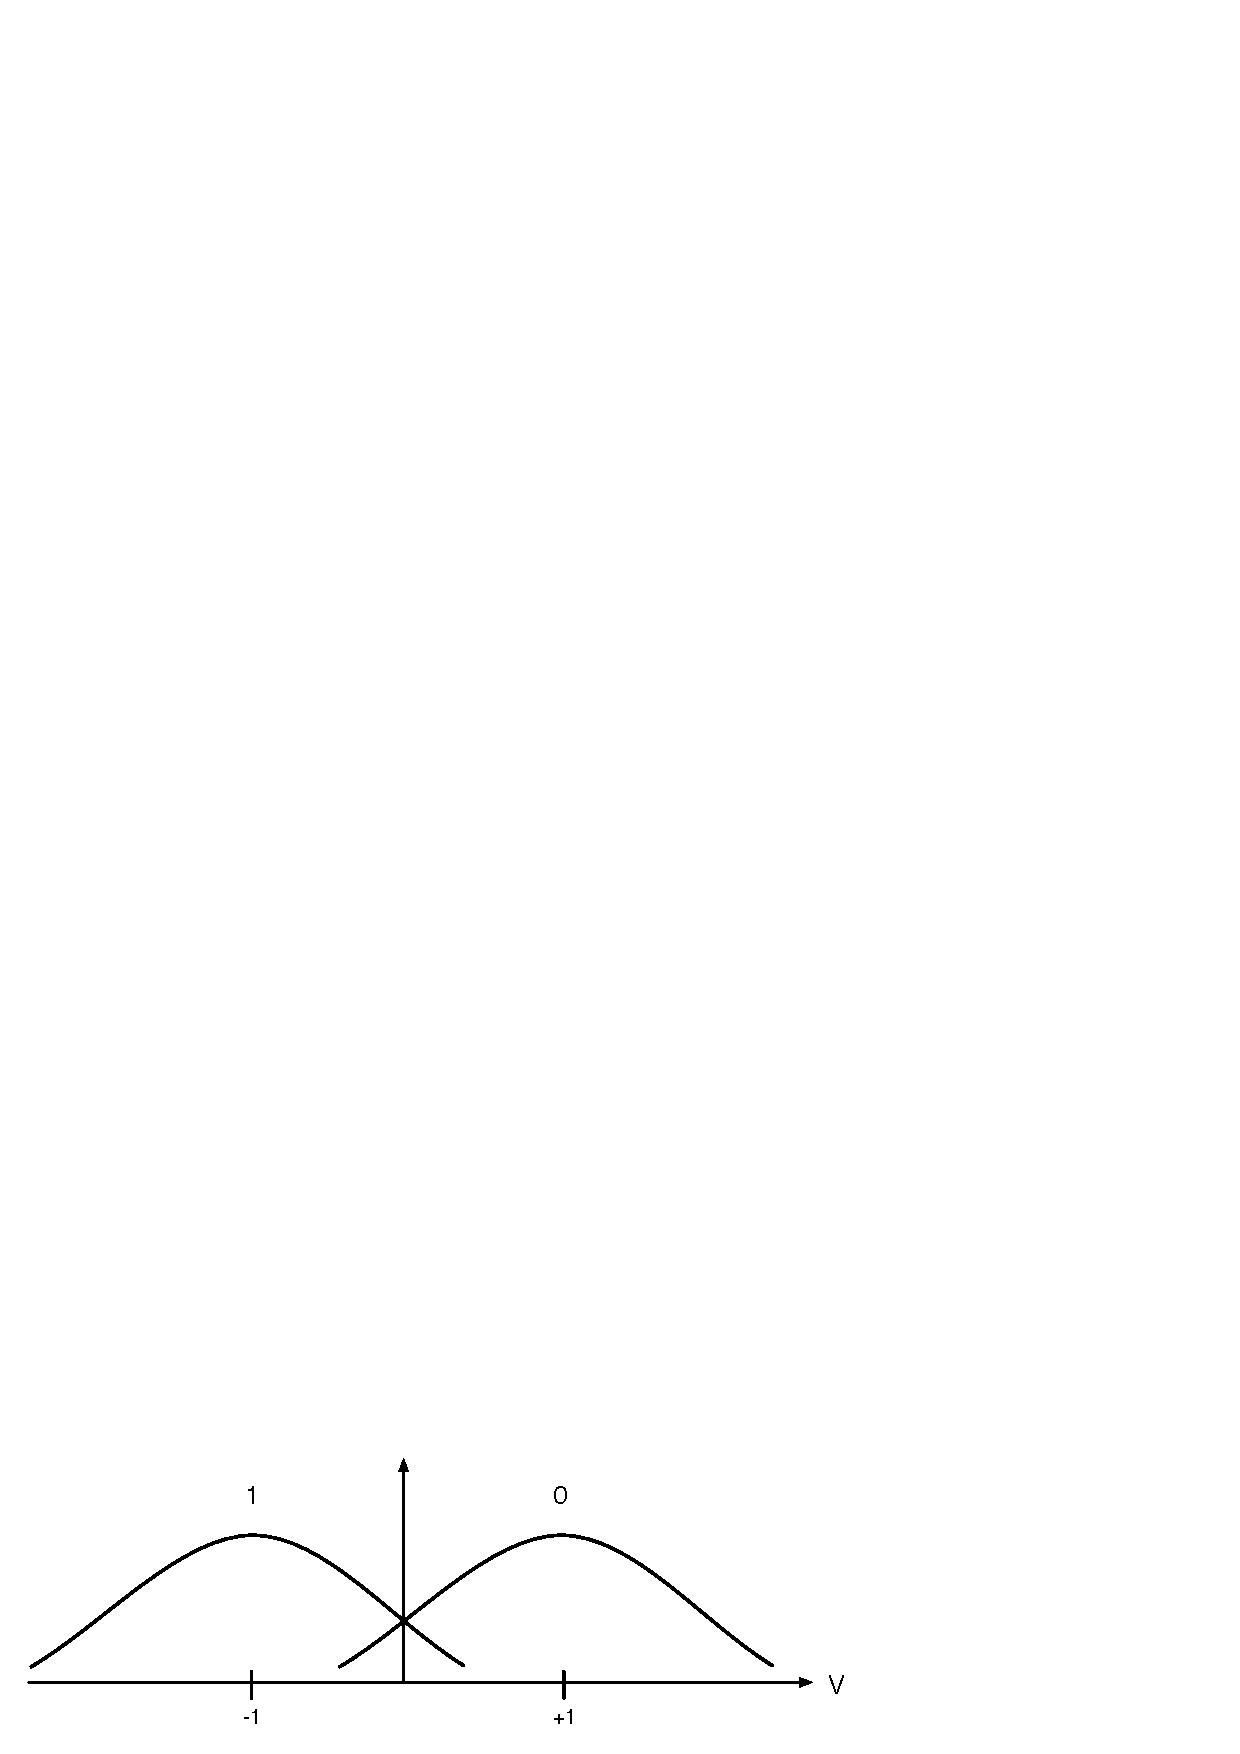
\includegraphics{BPSK_channel_graph}
\caption{Received voltage probability distribution for AWGN channel}
\label{figure:awgn probability graph}
\end{figure}

Figure \ref{figure:awgn probability graph} shows the typical probability distribution of a Binary Phase Shift Keying (BPSK) system with Additive White Gaussian Noise (AWGN). The x-axis is effectively a received voltage value from the demodulator. At transmission, a value of +1 volts corresponds to a binary 0, and a value of -1 volts corresponds to a binary 1. However, the additive noise in the channel results in the received voltage taking a range of values, and hence the received voltage is now defined as a probability distribution.

With hard decision decoding, the obvious boundary would be $x = 0$, half way between the +1 and -1 constellation symbols. Any value to the right side of this boundary would always be classified as binary 0, and anything to the left always binary 1. This means that a voltage value of 0.01 would be output as a binary 0, even though in practice it is almost equiprobable to be a binary 1. The fact that it could equally be a binary 0 or binary 1 is lost when making a hard decision, and the error correction decoder does not get that additional information.

Soft decision decoding seeks to improve on hard decision decoding, by making use of the actual received voltage value, rather than discarding it. The messages are now the conditional \textit{probabilites} of being a 1 or 0, instead of being just binary values. This allows the error correction decoder to know the degree of certainty that the message sent was a 1 or a 0.

\subsection{Hard decision decoding}
The message passing algorithm can be best understood with hard decision decoding. As an example, eq \ref{8,4 code} shows the parity check matrix $\mathbf{H}$ of an (8,4) code. This code can also be displayed, as in figure \ref{figure:tanner graph}, as a visual graph representation known as a tanner graph. [Reference: LDPC Leiner tutorial]

\begin{equation} \label{8,4 code} 
\mathbf{H} = 
\left(
\begin{array}{cccccccc}
  0 & 1 & 0 & 1 & 1 & 0 & 0 & 1 \\
  1 & 1 & 1 & 0 & 0 & 1 & 0 & 0 \\
  0 & 0 & 1 & 0 & 0 & 1 & 1 & 1 \\
  1 & 0 & 0 & 1 & 1 & 0 & 1 & 0 \\
\end{array}
\right)
\end{equation}

\begin{figure}[h]
\centering
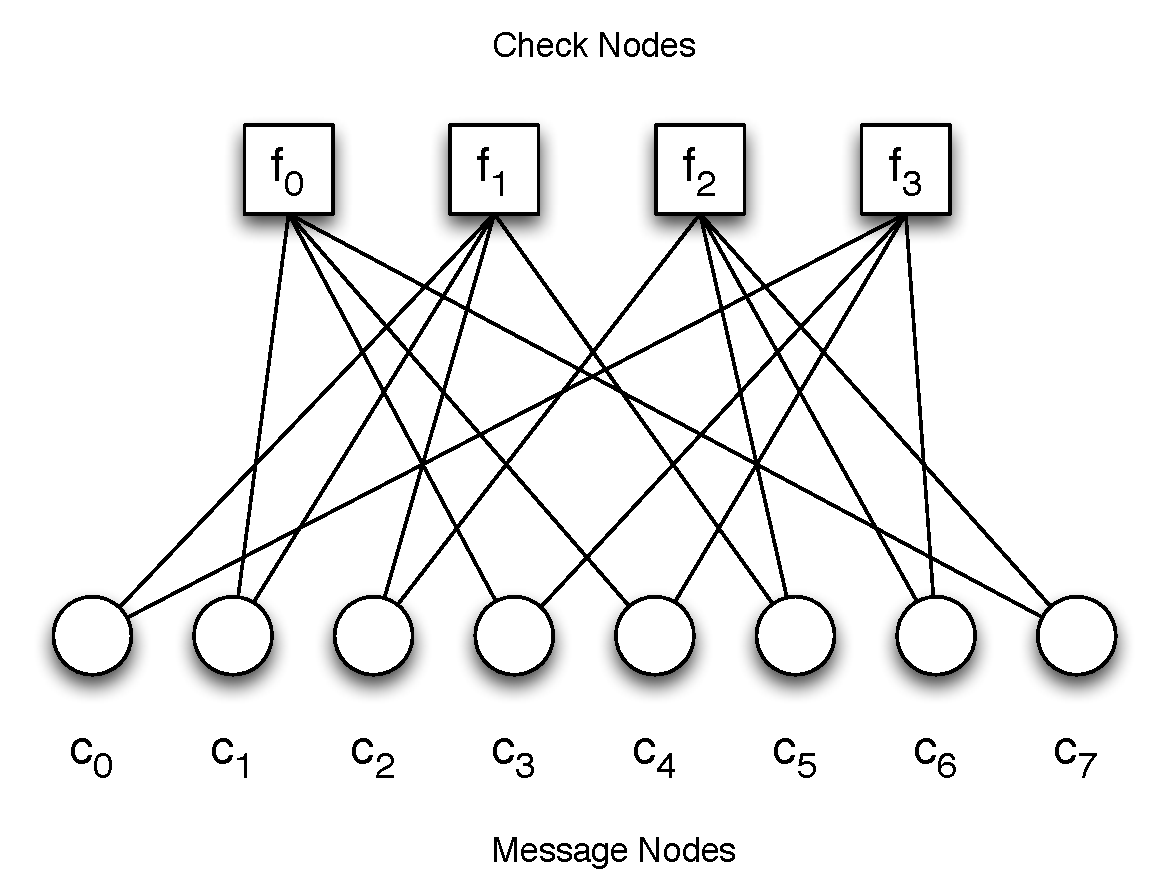
\includegraphics[scale=0.6]{tannergraph}
\caption{Tanner Graph}
\label{figure:tanner graph}
\end{figure}

The tanner graph is a bipartite graph with 2 types of node: Check nodes and Message nodes. The check nodes represent the $(n-k)$ parity check equations, whilst the message nodes represent the $n$ codeword bits. It is directly related to $\mathbf{H}$: Check node $f_j$ connects to message node $c_i$ if element $h_{ji}$ is $1$. Using the tanner graph, the hard decision decoding algorithm can now be explained as follows:
\begin{enumerate}
\item All message nodes $c_i$, having been initialised to the received codeword $y$, send their value to their connected check nodes $f_j$.
\item Each check node $f_j$ calculates a separate reply back to each message node $c_i$, with the binary value that it believes the message node should be. The parity check equation at each check node must satisfy $\lvert \sum f_j \rvert_{mod2} = 0$. From the example, check node $f_0$ receives values from $c_{1,3,4,7}$. When sending it's reply back to variable node $c_1$, it uses the values from nodes 3, 4 \& 7 along with the parity check constraint, to calculate the outbound message. Note that it does not use the information received from $c_1$ to send a reply back to $c_1$. This process continues: At each check node, a separate reply is calculated back to each connected message node.
\item The check nodes send their update back to the message nodes. Each message node in this example is connected to 2 check nodes, as well as having a previous value from step 1. As such, majority logic (with 3 bits in this case) can be used to decide whether the message node should be a 1 or a 0. 
\item The process now loops until the parity check constraint is satisfied for all nodes, at which the process terminates.
\end{enumerate}

\noindent A simple example describing the check node stage:
\begin{itemize}
\item Check node $f_0$ might receive values from $c_1$,$c_3$,$c_4$,$c_7$ = \{1,1,0,1\}.
\item To calculate the reply message to each $c_j$, use the parity check constraint $\lvert \sum f_0 \rvert_{mod2} = 0$:
\begin{itemize}
\item Reply for $c_1 : x + 1 + 0 + 1 = 0 \therefore c_1 = 0$ 
\item Reply for $c_3 : 1 + x + 0 + 1 = 0 \therefore c_3 = 0$ 
\item Reply for $c_4 : 1 + 1 + x + 1 = 0 \therefore c_4 = 1$ 
\item Reply for $c_7 : 1 + 1 + 0 + x = 0 \therefore c_7 = 0$
\end{itemize}
\item Repeat this process at all other check nodes $f_{1,2,3}$
\end{itemize}

\subsection{The Log-likelihood ratio} \label{section:LLR}
Whilst hard decision decoding is a good way to demonstrate how the iterative message passing algorithm works, soft decision decoding yields substantially better error correction performance, and is therefore the main method used in decoding LDPC.

In soft decision decoding, the message nodes no longer represent binary 1's or 0's, but instead can take a continuous range of probability values. These probability values are initially calculated using two sources of information: The received voltage value of each bit, and the underlying probability distribution of the received bit. Before being able to describe the soft decision decoding algorithm, this information needs to be formed into a useful metric: the \textit{Log-likelihood ratio}, [Reference: LLR computation.pdf]

\begin{equation} \label{eq:LLR}
\mathcal{L}(c|y) = log_e \left[ \dfrac{f(c=+1|y)}{f(c=-1|y)} \right]
\end{equation}

\noindent The term $\mathcal{L}(c|y)$ is the likelihood of $c$ being transmitted given that $y$ was received. The log-ratio is able to tell us if $c=+1$ or $c=-1$ was the most likely transmitted symbol, given the received value $y$. A positive LLR indicates it is more likely that $c=+1$ was transmitted, and a negative LLR that $c=-1$ was transmitted. Additionally, the LLR has a range of $-\infty$ to $+\infty$, which provides the degree of certainty of a given symbol.

To make use of the LLR, it is necessary to manipulate it into a more useful form. Using Bayes' rule\footnote{$P(A|B) = \dfrac{P(B|A) P(A)}{P(B)}$}, and the assumption that the transmitted bits are equiprobable\footnote{i.e. $f(c=+1) = f(c=-1)$},

\begin{equation}
\begin{aligned}
\mathcal{L}(c|y) &= log_e \left[ \dfrac{f(y|c=+1) \dfrac{f(c=+1)}{f(y)}}{f(y|c=-1) \dfrac{f(c=-1)}{f(y)}} \right] 
\\
&= log_e \left[ \dfrac{f(y|c=+1)} {f(y|c=-1)} \right] 
\\
&\sim log_e \left[ \dfrac{\text{\textit{``Probability density function of +1"}}}{\text{\textit{``Probability density function of -1"}}} \right]
\end{aligned}
\end{equation}

\noindent The LLR can now be calculated for each received value of $y$. Note that it is necessary to have the underlying density functions of the received symbols. By inserting the received value $y$ into each PDF, you obtain a numerical probability of $y$ representing either +1 or -1. The ratio of these 2 probabilities then gives us the likelihood ratio.

The LLR method applies in general to all noisy channels, that is, the probability density functions can take any form. However when dealing with the AWGN channel, converting from a received symbol amplitude $y$ into the LLR is much simpler, since the probability density function in both cases is a gaussian,

\begin{equation} \label{eq:LLR_awgn}
\begin{aligned}
\mathcal{L}(c|y) &= log_e \left[ \dfrac{\mathcal{N}(1,\sigma^2)} {\mathcal{N}(-1,\sigma^2)} \right] 
\\
&= log_e \left[ \dfrac{e^{-(y-1)^2/(2\sigma^2)}}{e^{-(y+1)^2/(2\sigma^2)}} \right]
\\
&= log_e \left[ e^{4y/(2\sigma^2)} \right]
\\
&= \dfrac{2y}{\sigma^2}
\end{aligned}
\end{equation}

\noindent This result makes it very easy to take the output from the demodulator (the +1/-1 BPSK $y$ symbols) and generate the appropriate LLR's for the AWGN channel.

\subsection{Soft decision decoding}
The Belief Propagation algorithm for soft decision decoding follows a similar process to that of hard decision decoding. Messages are passed between check and variable nodes defined by the tanner graph. The main difference is what happens at each of the nodes, since now the messages are LLR's rather than binary bits. 

[Papers such as ??, ?? and ??] have all proved the set of equations that are used at both the message nodes and check nodes. The belief propagation algorithm can be distilled into just 2 equations: The message node update equation, and the check node update equation. The reason why it is often called the 'Sum-Product' algorithm, is since the message node update equation involves summing the LLR's, and the check node update equation involves taking their product.

\begin{equation} \label{eq:msgNode}
m_{ij}^{(l)} = L_i+\sum\limits_{j'\in C_i \ne j}m_{j'i}^{(l-1)}
\end{equation}

Equation \ref{eq:msgNode} is the message node update equation. $m_{ij}^{(l)}$ is the message sent from message node $i$ to check node $j$, at iteration $l$. $L_i$ is the initial LLR for message bit $i$. The expression $j'\in C_i \ne j$ is used to sum the incoming messages from all check nodes $j'$ that are connected to $C_i$, except the current node $j$ that is being sent to. This exclusion is the same as for hard decision decoding, whereby a message to a node is never a function of a message from that node (the extrinsic information rule). Finally, $m_{j'i}^{(l-1)}$ indicates that the sum is of the received check node messages from the last ($l-1$) iteration.

\begin{equation} \label{eq:chkNode}
m_{ji}^{(l)} = 2\arctanh\left[\prod\limits_{i'\in V_j\ne i} \tanh(\dfrac{m_{i'j}^{(l-1)}}{2})\right]
\end{equation}

Equation \ref{eq:chkNode} is the check node update equation. $m_{ji}^{(l)}$ is the message sent from check node $j$ to message node $i$, at iteration $l$. As before, $i'\in V_j\ne i$ includes all message nodes $i'$ that are connected to check node $V_j$, except the current node $i$ that is being sent to (extrinsic information rule).

\noindent With both node equations defined, the iterative soft decision decoder proceeds as follows:

\begin{enumerate}
\item All message nodes $c_i$, having been initialised to the received LLR's $L_i$, send their value to their connected check nodes $f_j$. 
\item At each check node $j$, using equation \ref{eq:chkNode}, the return message to each connected message node $i$ can be calculated.
\item Sum the LLR's received at each message node, and obtain the binary value of the codeword ($l_i > 0 \rightarrow 0$, $l_i < 0 \rightarrow 1$). Using the parity check equation $\mathbf{s=c H}^\top$, where $c$ is the current binary value of the codeword, we obtain the syndrome. If the syndrome is all-zero, the algorithm terminates, since a valid (though not necessarily correct) codeword $c$ has been found.
\item At each message node $i$, using equation \ref{eq:msgNode}, the return message to each connected check node $j$ can be calculated.
\item Steps 2-4 repeat until a valid codeword is found, or up to a maximum number of iterations (Usually around $l=50$). 
\end{enumerate}

\subsection{Min-Sum approximation}

Min sum to go here (0.5 pages)

\section{The AWGN channel: Simulation \& Results}
One of the most important noisy channels used in communications theory, and already mentioned previously, is the Additive White Gaussian Noise (AWGN) channel. Whilst this noise channel is not really applicable to model Flash Memory, which is the aim of this project, it is however a useful benchmarking tool to ensure that the MATLAB decoder is working correctly. It is also a good method of demonstrating the power of LDPC, soft decision decoding, and error-correcting codes generally. This section presents the work done in modelling the encoder, AWGN channel, and decoder, and compares the results to known data sets.

\subsection{Simulation model}
\begin{figure}[h]
\centering
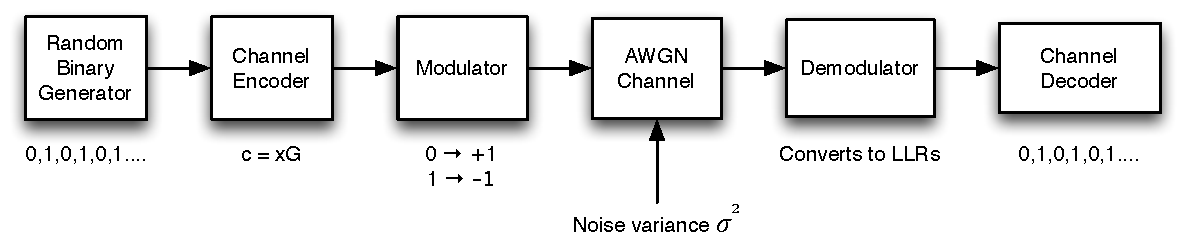
\includegraphics[scale=0.878]{awgn_channel_model}
\caption{The AWGN simulation model}
\label{figure:awgn sim model}
\end{figure}

\begin{itemize}
\item The random generator produces a vector of pseudo-random, uniformly distributed values from the set \{1,0\}, of length $k$.
\item The channel encoder takes the length $k$ message, and encodes it using the generator matrix, into a block of length $n$.
\item The modulator maps each binary bit, in this case using Binary Phase-Shift Keying (BPSK), onto a constellation symbol. These symbols represent a real voltage value.
\item The channel is simulated by adding white gaussian noise onto each symbol. The output from the channel is $\mathbf{Y = X + N}$, where $\mathbf{X}$ is the input random variable (+/- 1), and $\mathbf{N}$ is the noise random variable ($\mathbf{N} \sim \mathcal{N}(0,\sigma^2)$)
\item The demodulator, for soft decision decoding, calculates the LLR of each received symbol. From equation \ref{eq:LLR_awgn}, $\mathcal{L} = \dfrac{2y}{\sigma^2}$, where $y$ is the received value from the output of the channel, and $\sigma^2$ is the AWGN channel noise variance. In a real system, this method therefore requires knowledge of the underlying noise parameters. For the simulation, the value is assumed to be known.
\item Finally, the channel decoder performs error correction using the Belief Propagation algorithm, and outputs the corrected codeword (Note: The encoded message can be extracted from the codeword if a systematic generator matrix was used).
\end{itemize}

To simulate the error correction performance of this system, and compare it to other results, there needs to be a standardised quantity to describe the error rate and the channel noise. Whilst the noise variance is one such quantity, it doesn't take into account the relative difference between signal power and noise power. A far more useful metric would be Signal-to-noise ratio (SNR), or more specifically in this case $\dfrac{E_b}{N_0}$ (energy per bit/noise power). Like SNR, this is usually given in decibels\footnote{For the conversion calculations, $\dfrac{E_b}{N_0}$ must be a linear, not logarithmic, value. i.e: $\dfrac{E_b}{N_0}(\text{dB}) = 10\log_{10}\left[\dfrac{E_b}{N_0}(\text{lin})\right]$}. 
\vspace{3mm} \\
\noindent
Converting between $\sigma^2$ and $\dfrac{E_b}{N_0}$ is relatively trivial:
\vspace{3mm} \\
\noindent
\begin{tabular}{lcl}
$E_s$ & - & Energy per symbol (Always 1 for BPSK) \\
$R_c$ & - & Code rate \\
$R_m$ & - & Modulation rate (Always 1 for BPSK) \\
$E_b$ & - & Energy per information bit \\
\end{tabular}
\begin{equation} \label{eq:noisePwr}
\sigma^2 = \dfrac{N_0}{2}
\end{equation}
\begin{equation}\label{eq:EnergyperSymbol}
E_s = R_cR_mE_b
\end{equation}
$N_0$, the noise power, is defined as in \ref{eq:noisePwr}. The energy per symbol is defined in \ref{eq:EnergyperSymbol}: the energy per bit multiplied by both the number of bits per symbol and the ratio of useful message data. By substituting $E_s$ into $\dfrac{E_b}{N_0}$:
\begin{equation}
\begin{aligned}
\dfrac{E_b}{N_0} &= \dfrac{E_s}{R_cR_mN_0} \\
&= \dfrac{E_s}{R_cR_m2\sigma^2} \\
&= \dfrac{1}{2R_c\sigma^2}
\end{aligned}
\end{equation}
$E_s = R_m = 1$ in this case, further simplifying the equation. This allows the conversion between $\sigma^2$, the parameter used in the noise model, and $\dfrac{E_b}{N_0}$, the metric used to present the results.

The dependent variable in the simulation is the Bit Error Rate (BER). The output from the channel encoder is compared to the output from the channel decoder, where both are blocks of length $n$. The number of bit errors is simply the difference between the two codewords (similar to the Hamming distance). This raw bit error number is then divided by the block length, to obtain a bit error rate.

Each instance of the block diagram in figure \ref{figure:awgn sim model} generates a random binary block, and the noise added to that block is also random. A single sample will not be sufficient to get an accurate error rate of the system for a given noise value, since at very low error rates thousands of blocks may need to be decoded before a single bit error occurs. Performing a simulation of repeated sampling is known as a Monte Carlo simulation. The process in MATLAB is therefore designed to perform $N$ trials of the simulation, with each trial outputting a bit error rate. After completing all trials, the bit error rate can be averaged over all blocks. In this project, for the lowest bit error rate experiments, up to $10^6$ blocks were processed per noise value.

\subsection{Simulation results}
\begin{figure}[h]
\centering
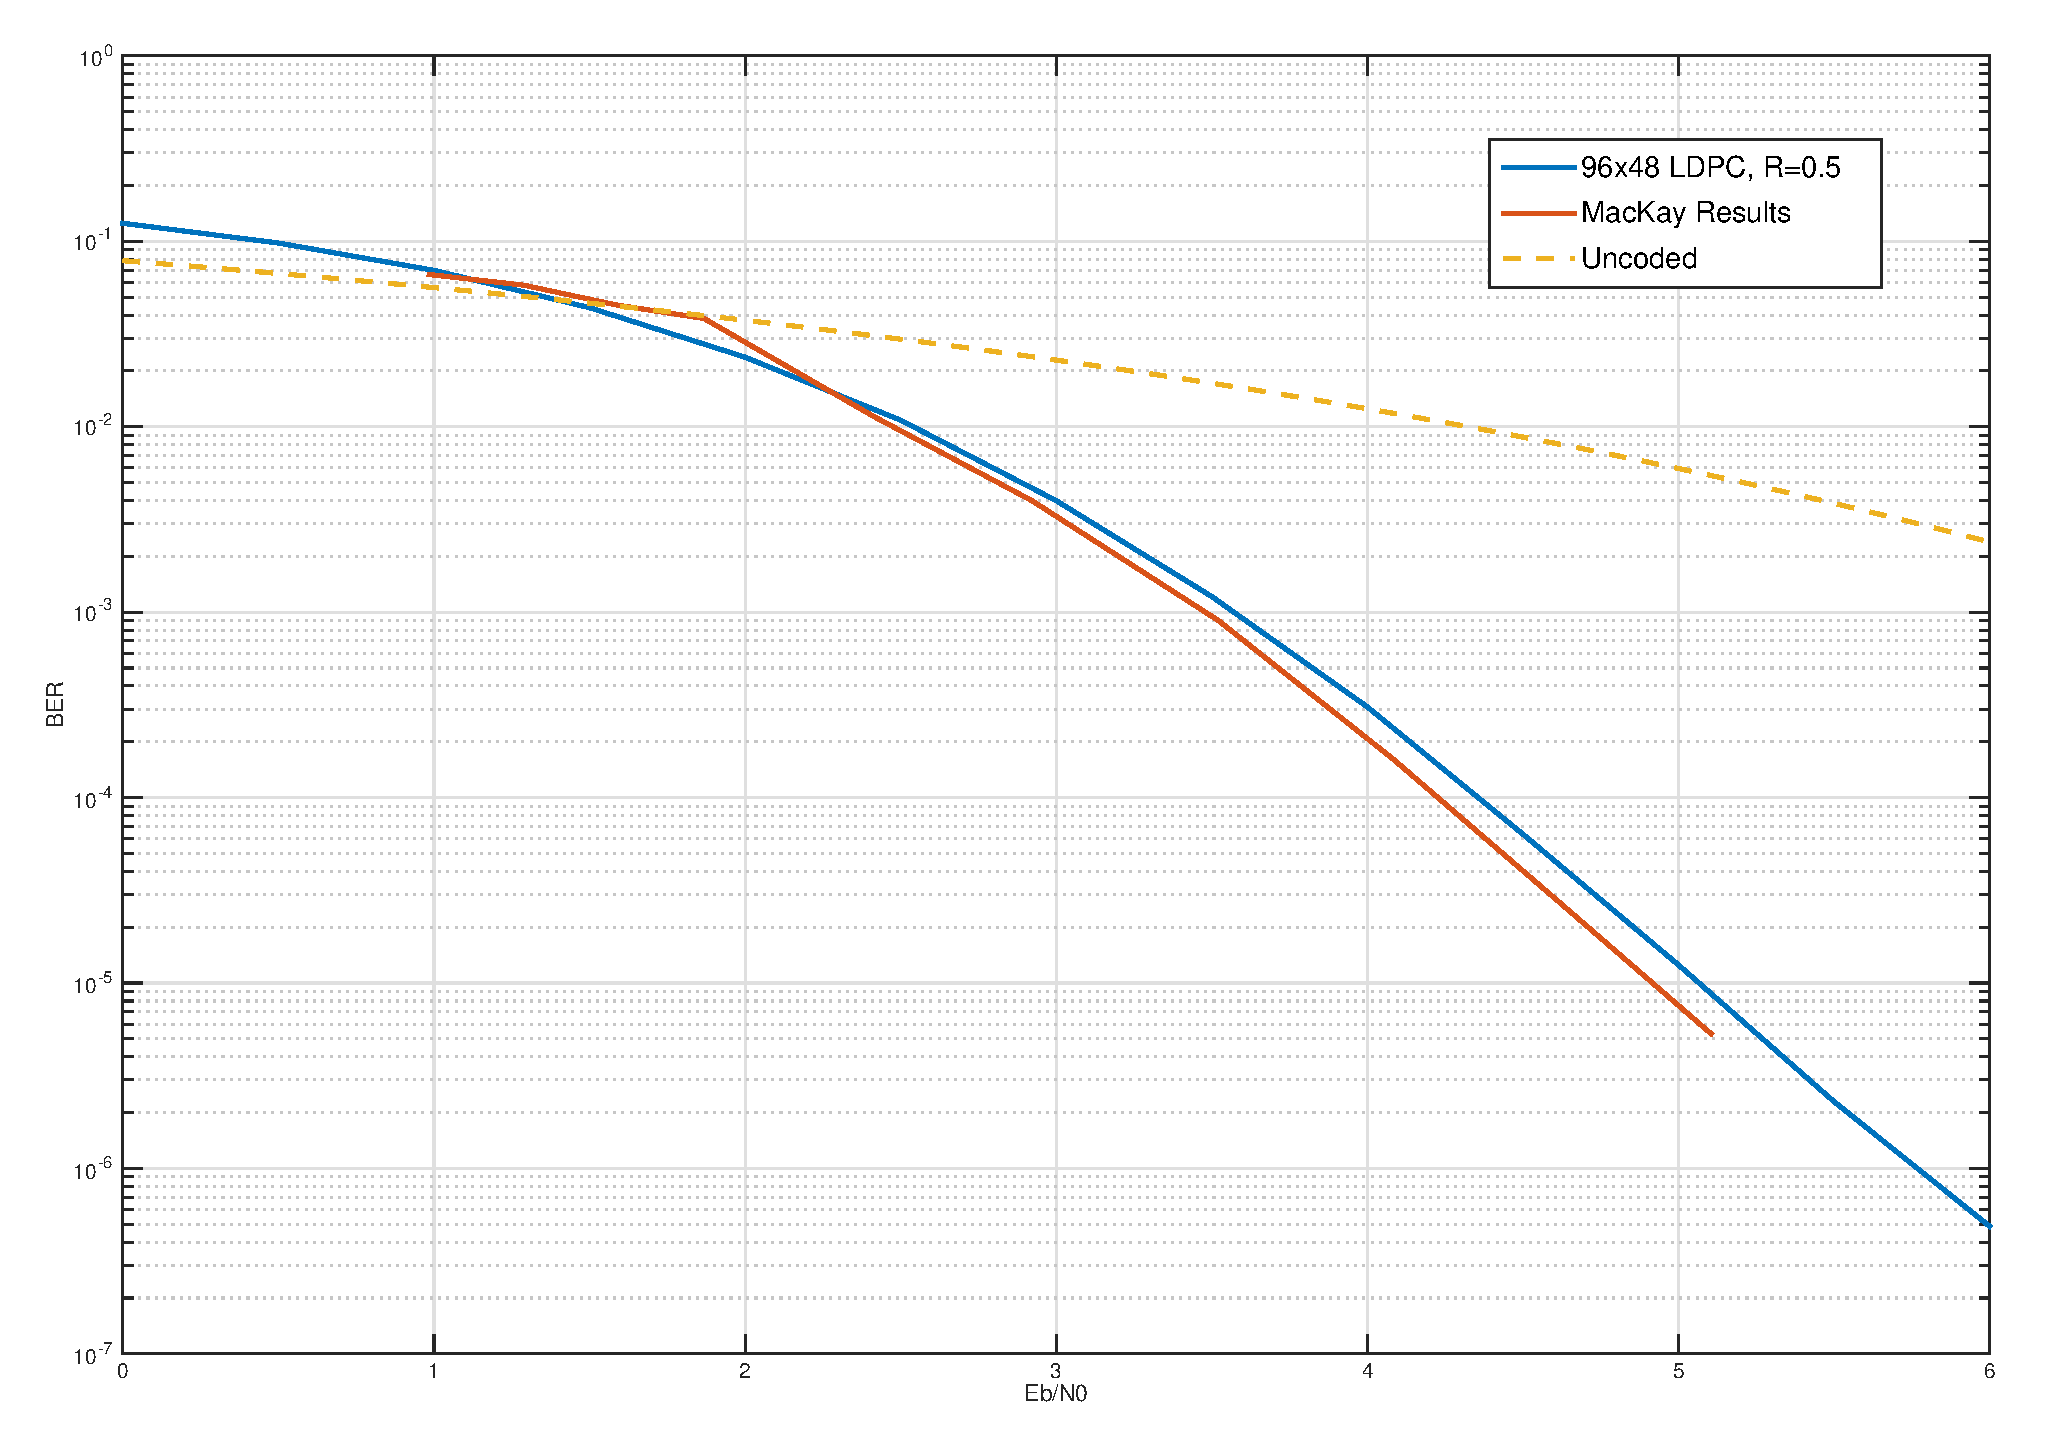
\includegraphics[scale=0.5]{96_48_LDPC}
\caption{Simulated results of 96,48 LDPC code}
\label{figure:96_48_LDPC_graph}
\end{figure}

A short block length, rate $\dfrac{1}{2}$ LDPC code was used to produce the results in figure \ref{figure:96_48_LDPC_graph}, using the Sum-Product algorithm with soft decision decoding. The figure also displays the results obtained by MacKay using the same LDPC code and decoding method. There is a minor performance loss compared to MacKay, but otherwise the results are in agreement. Additionally, the dashed line indicates the expected bit error rate in the event that no error correction code was used. There is therefore a substantial coding gain in this system, for example to achieve a BER of $10^{-6}$ requires around $5.5$ dB with coding, and nearly $10$ dB without.

\begin{figure}[h]
\centering
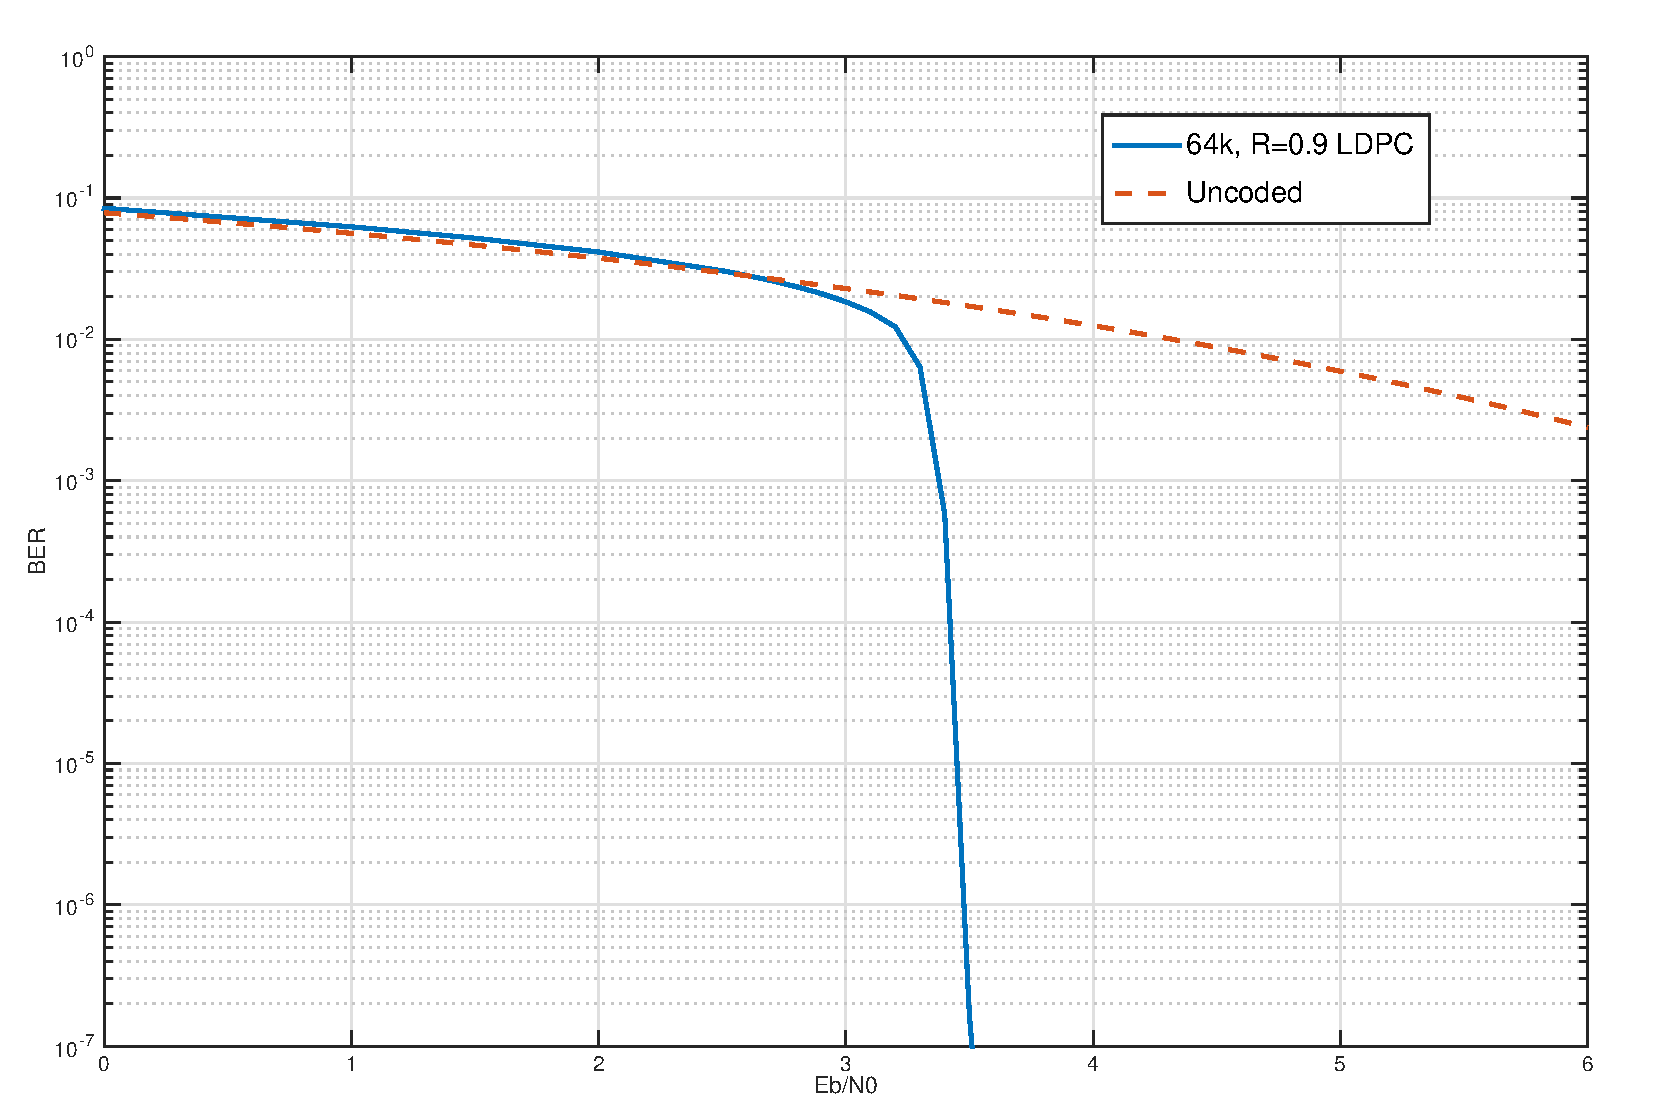
\includegraphics[scale=0.6]{dvbs2_graph}
\caption{Simulated results of 64k DVB-S2 LDPC code}
\label{figure:64k_LDPC_graph}
\end{figure}

Longer block length codes generally achieve superior performance and greater 'cut-off' compared to shorter codes. Figure \ref{figure:64k_LDPC_graph} demonstrates a code with a block length of $64000$, and a substantially higher rate ($R=0.9$). This particular code is a standardised construction, used in the DVB-S2 (Satellite broadcasting) specifications. This code is also the primary one used in this project for the memory error correction later. One benefit of using this code is its sharp 'cut-off', compared to the previous code in figure \ref{figure:96_48_LDPC_graph}.

\subsection{Conclusion}
Simulating the AWGN channel, and then comparing the results to the known data published by MacKay, allows for some degree of verification of the MATLAB program. The AWGN channel is one of the common channels simulated when dealing with error correcting code, since it simulates the effect of random noise that often occurs in the environment. 

One issue identified with the simulation program was the speed of the decoder. In the first version of the decoder program [?? Matlab appendix section], there were a substantial number of 'for' loops, which are generally slow in MATLAB. Subsequent versions of the decoder attempted to fix this by vectorising the code [?? Matlab appendix section 2], resulting in approximately a 4x speed increase. However, even with these improvements, the decoder was still much slower compared to MATLAB's built-in LDPC decoder [?? matlab reference page]. In addition, freely available OpenCL accelerated decoders [?? openCL ref] can be used on a GPU (Graphics Processing Unit) which are even faster than MATLAB's implementation (See appendix [??] for the benchmark comparisons). In the subsequent sections simulating the memory model, the MATLAB built-in implementation of the LDPC decoder was used, allowing for substantially more blocks to be decoded in the same amount of time.

\section{Modelling a memory-specific noise channel}
There are many similarities between modelling a communications system and flash memory. Both are binary channels, subject to some binary input, distortion by some noise source, and subsequent decoding. However, the major difference in flash memory is the storage of binary data in the device for a length of time, unlike a communications system where the data is 'in transit'. When a bit is stored to a memory cell, the noise effect is cumulative over the lifetime of the stored bit. Therefore, two major parameters in modelling flash memory are time, and the number of read/write (or Program/Erase) cycles each cell is subject to.

As stated previously in section \ref{section:memtech}, it is the threshold voltage of each gate that defines the binary value of the memory cell. In this project, the flash memory is assumed to be of SLC design, that is 1 bit per cell. It is also assumed that a low gate threshold voltage corresponds to a binary 0, whilst a higher threshold voltage corresponds to a binary 1. 

The primary noise source, which is caused by repeated P/E cycling, can be split into two physical phenomena: Electron capture and emission events, which result in a random variation of the threshold voltage, and interface trap recovery and electron de-trapping, which gradually reduces the gate threshold voltage over time. The former is known as `Random Telegraph Noise' (RTN), whilst the latter is often called the `Retention Noise', since it sets a time limit on how long data can be stored in a cell until the threshold voltage becomes too low.

Another noise source, known as `Cell-to-cell interference', which as the name implies is the result of neighbouring memory cells interfering with each other. This dependence between neighbouring cells adds additional complexity when modelling the system, since it is no longer possible to model one cell at a time. As a result, it was decided for this project not to include this noise source, instead focusing on an individual memory cell.

\subsection{Description of Noise Sources}

The first noise source in the memory channel, the random telegraph noise (RTN), can be modelled as a Laplacian distribution, $Y_{rtn} \sim \mathcal{L}(\lambda_{rtn})$, whose probability density function is
\begin{equation} \label{eq:RTN}
p_{rtn}(x) = \dfrac{1}{2\lambda_{rtn}}e^{-\lvert x \rvert / \lambda_{rtn}}
\end{equation}
In equation \ref{eq:RTN}, $x$ is the value of the voltage fluctuation, and $\lambda_{rtn}$ scales with $N$, the P/E cycling number. In this project, $\lambda_{rtn} = K \sqrt{N}$ where $K$ is just a constant. Therefore as the memory cell is subject to more P/E cycles ($N$), the RTN distribution widens, as expected. Figure \ref{figure:RTN_graph} shows the probability density function of the distribution for different values of $N$. The distribution is centered about $x=0$, since the random effect of RTN can result in either an increase of decrease of the cell threshold voltage.

\begin{figure}[h]
\centering
\minipage{0.5\textwidth}
\centering
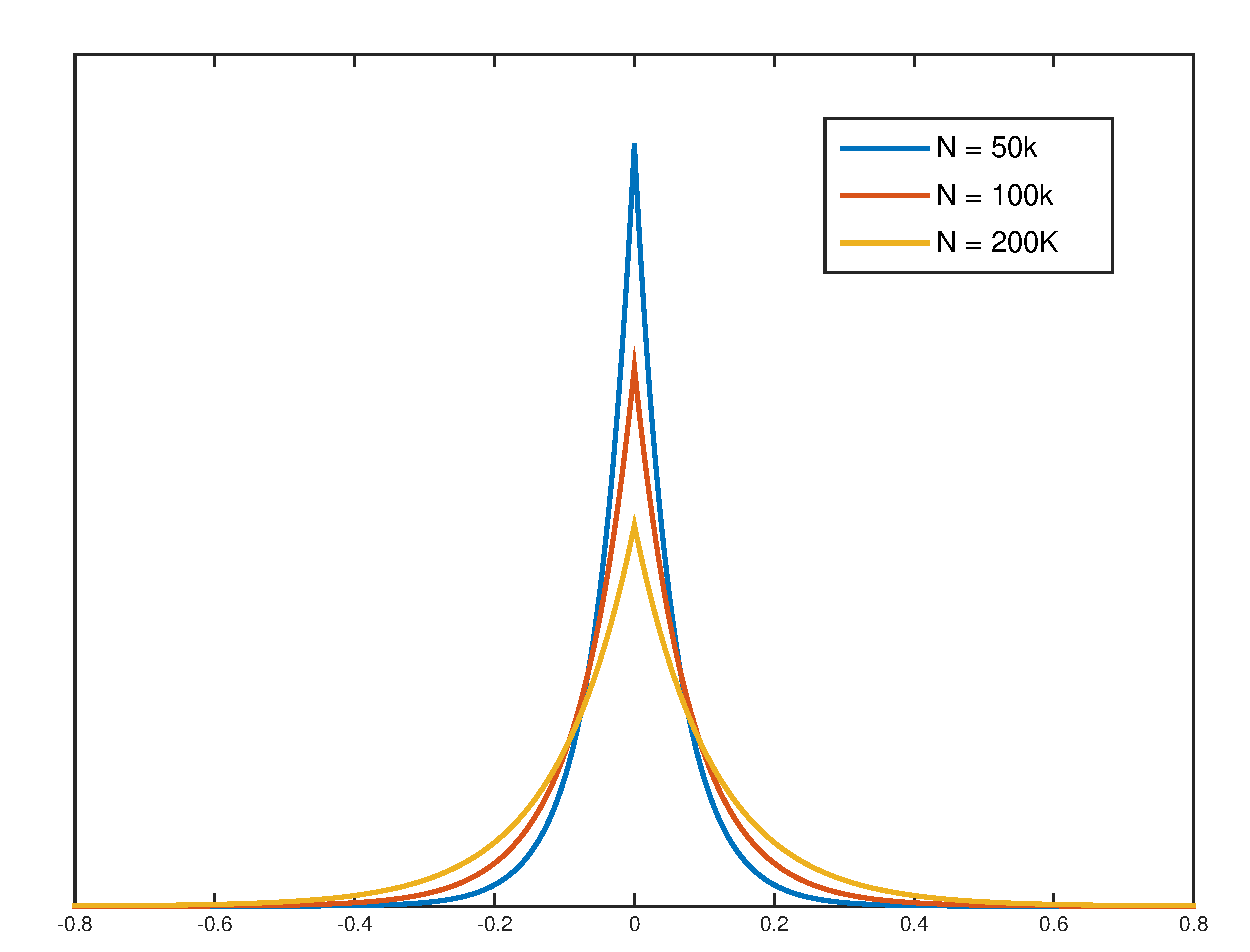
\includegraphics[scale=0.42]{RTN_graph}
\caption{PDF of RTN distribution}
\label{figure:RTN_graph}
\endminipage\hfill
\minipage{0.5\textwidth}
\centering
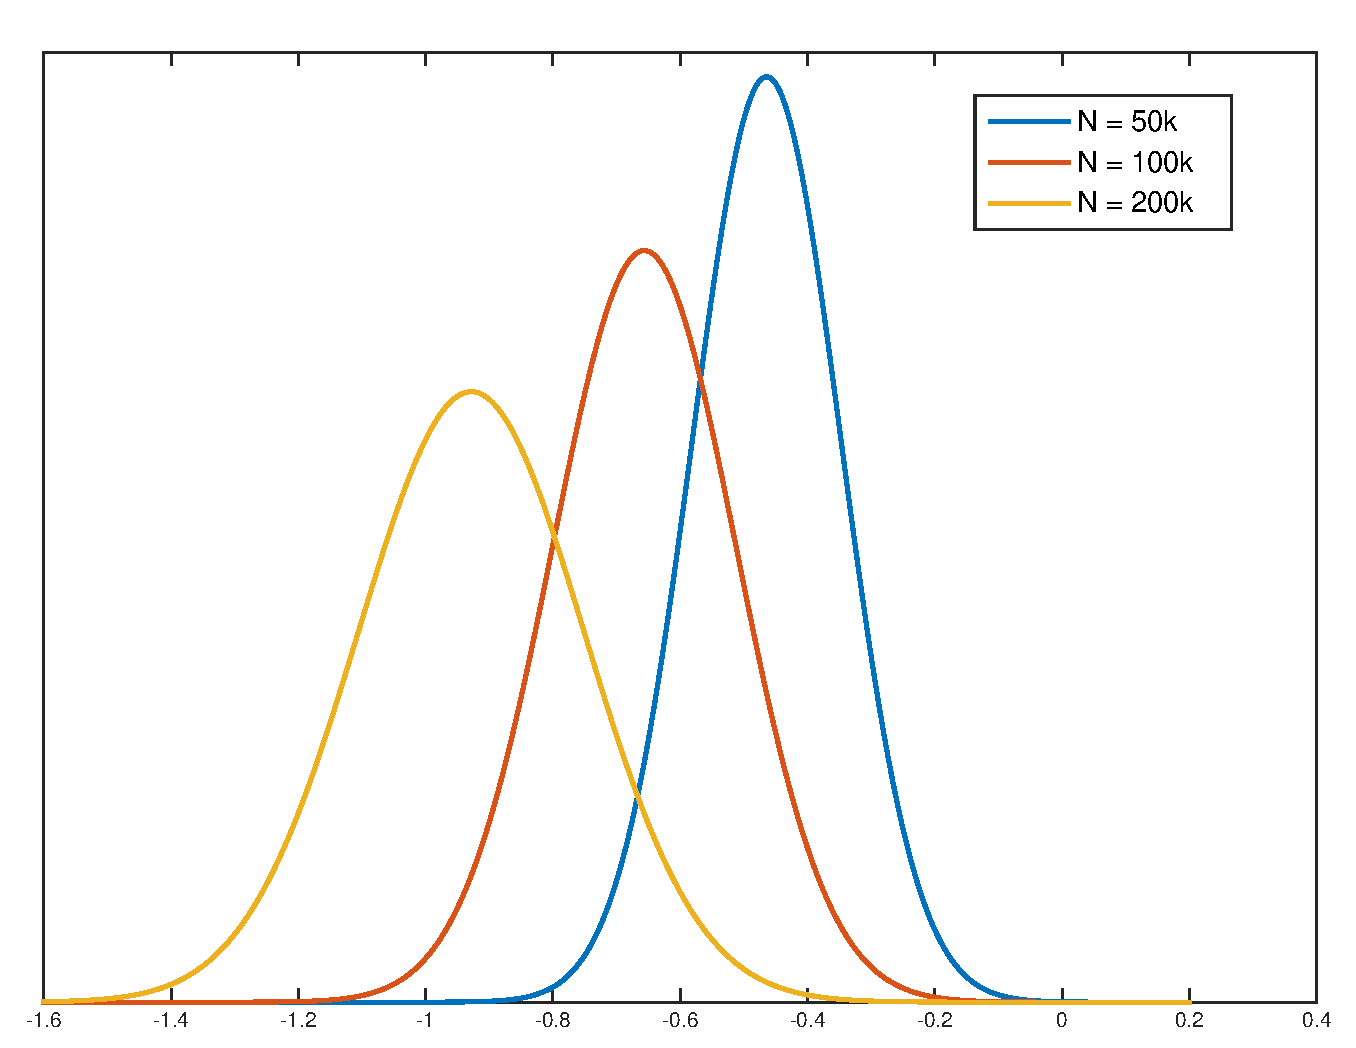
\includegraphics[scale=0.378]{retention_noise_graph}
\caption{PDF of Retention noise distribution}
\label{figure:ret_graph}
\endminipage
\end{figure}

The second noise source, the retention noise, is modelled as a Gaussian, $Y_{retention} \sim \mathcal{N}(\mu_r,\sigma_r^2)$, with the mean and variance defined as
\begin{equation} \label{eq:retention}
\begin{aligned}
\mu_r &= -K_sK_d(V_p-V_e)N^{0.5}\ln\left(1+\dfrac{t}{t_0}\right)\\
\sigma_r^2 &= K_sK_m(V_p-V_e)N^{0.6}\ln\left(1+\dfrac{t}{t_0}\right)
\end{aligned}
\end{equation}
In equation \ref{eq:retention}, $V_p$ is the initial voltage of the programmed state, $V_e$ is the (mean) voltage of the erased state, $t$ is the current memory retention time, and $t_0$ is an initial starting time. $K_{s,d,m}$ are all constants. The retention noise therefore has a power-law relationship with the P/E cycling number $N$, a logarithmic relationship with retention time, and is also dependent on the initial threshold voltages. Figure \ref{figure:ret_graph} shows the probability density function of the retention noise for different values of $N$, with the remaining variables fixed. Also note that since the mean ($\mu_r$) is always negative, the effect of the Retention noise is to always reduce the gate threshold voltage. As $N$ increases, the programmed state voltage will therefore reduce and get closer to the erased state voltage. This is perhaps the main source of bit error: the interference between the erased and programmed states. 

\subsection{Channel Model} \label{section:memory_channel_model}
Both the RTN and retention noise are independent random variables. Therefore the threshold voltage of any given cell is simply the sum of the random variables. As explained previously in section [??], each cell is either a binary 0 or 1, with a corresponding threshold voltage distribution for each. Therefore in the ideal case each cell will have a single voltage value, either $V_{p_0}$ for a programmed cell or $V_{e_0}$ for an erased cell. After noise, the final threshold voltage of the cell is then

\begin{equation} \label{eq:additive_memory_noise_model}
\begin{aligned}
V_{p} &= V_{p_0} + Y_{rtn} + Y_{retention} \\
V_{e} &= V_{e_0} + Y_{rtn}
\end{aligned}
\end{equation}
where $V_{p}$ and $V_{e}$ are the final programmed and erased voltage states, respectively. Retention noise is not added onto the erased state in this model, since we are assuming that the erased state is the reference voltage level that the retention noise is derived from.
\bigskip

\begin{figure}[h]
\centering
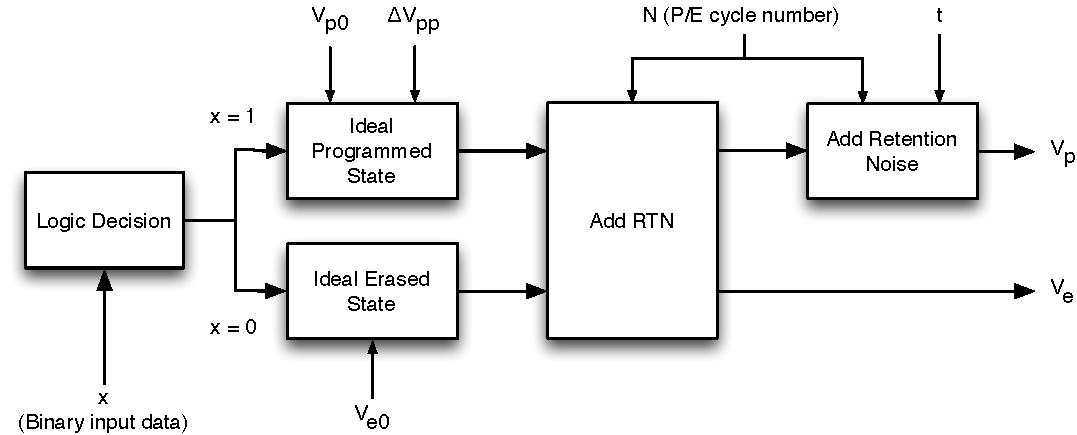
\includegraphics[scale=0.96]{memory_channel}
\caption{Memory channel noise model}
\label{fig:mem_channel_model}
\end{figure}

Figure \ref{fig:mem_channel_model} shows the block diagram of the memory channel noise model. Unlike the AWGN channel, the noise added to each binary bit depends on whether it is a 0 or a 1. The input to the model is a binary value, whilst the output from the model is the final threshold voltage value of the memory cell, ready to be decoded. Effectively, the model simulates the programming of a memory cell, and then the subsequent noise that would be experienced if the cell were subjected to repeated program and erase cycles.

\begin{figure}[!ht]
\centering
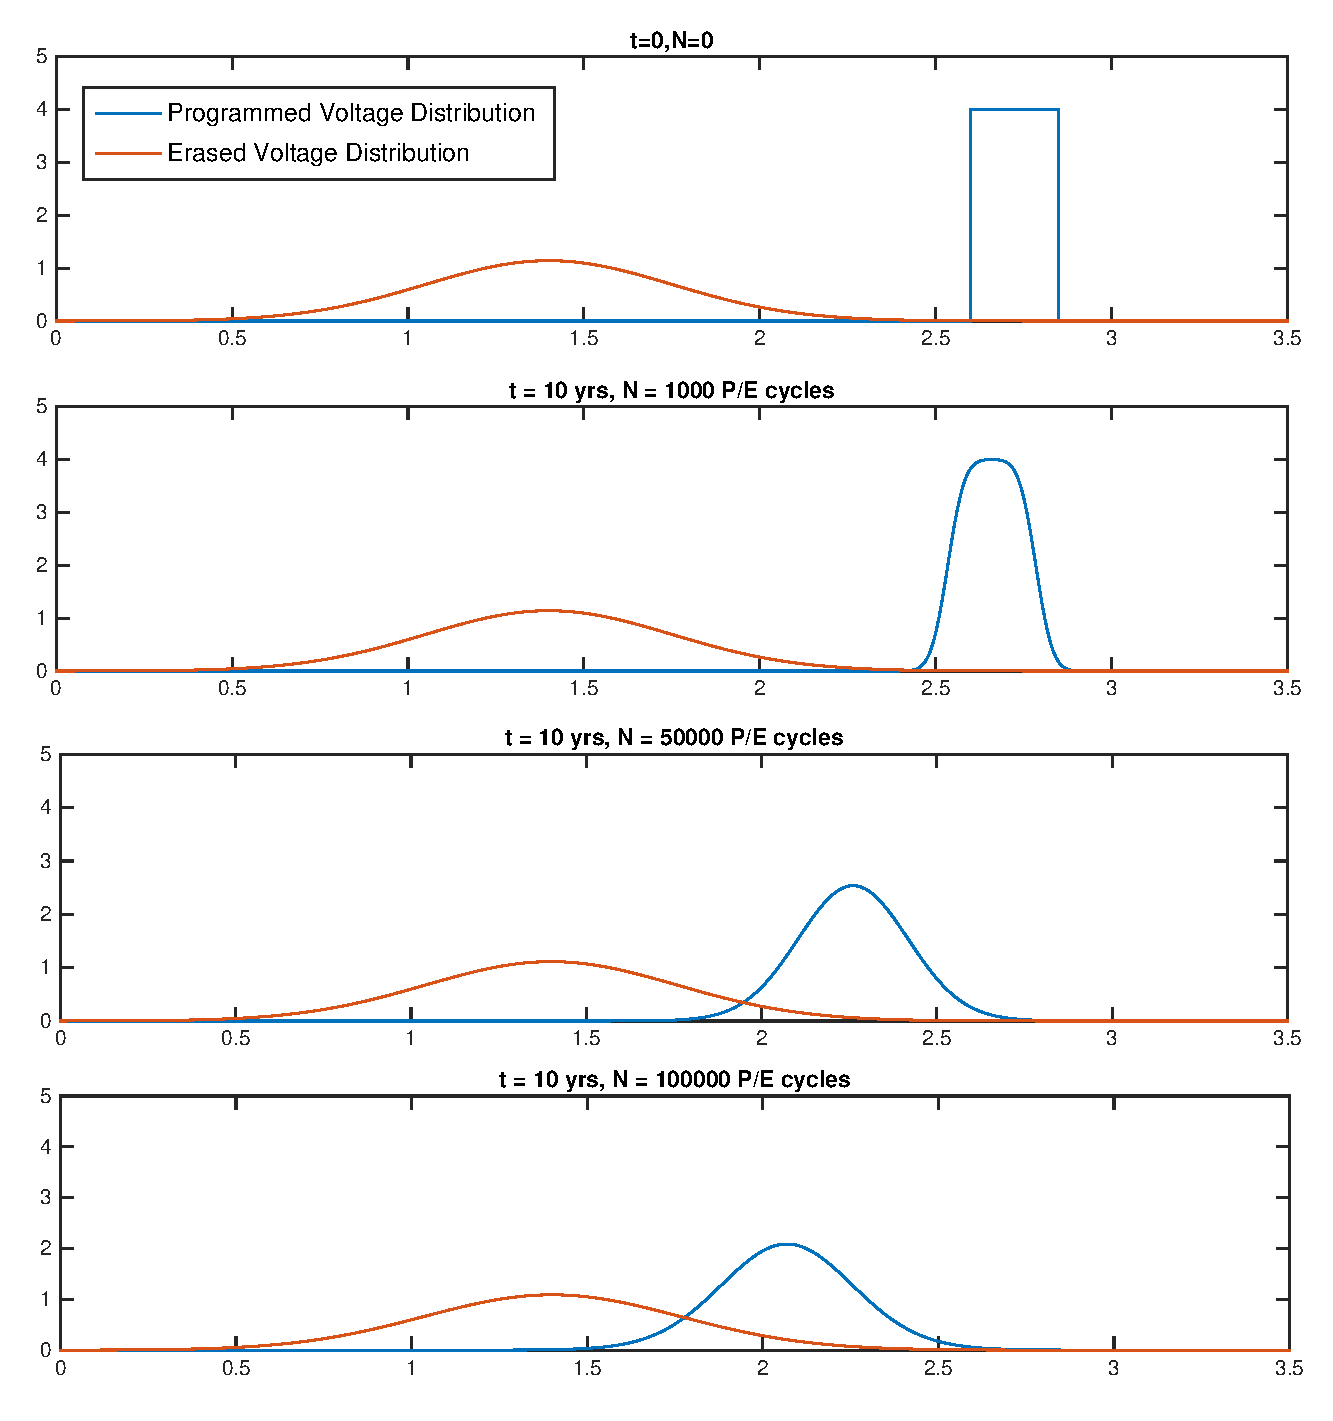
\includegraphics[scale=0.75]{memory_voltage_distribution}
\caption{Density functions of memory threshold voltages for differing values of N}
\label{fig:mem_channel_distribution}
\end{figure}

Figure \ref{fig:mem_channel_distribution} shows the probability density functions obtained from the memory model in figure \ref{fig:mem_channel_model}. Note that the $x$ axes are the gate threshold voltages. Various values for $N$ are displayed as well as showing the initial programmed state (the uniform distribution) when $N=0$. As the number of P/E cycles increases, the programmed distribution shifts left and widens, and interferes with the erased state. It is now clear that a simple hard-decision decoder without any error correction would generate a substantial number of errors when, in this case, $N > 50,000$. The distributions overlap, which would lead to incorrectly decoded bits.

\section{Decoding for the memory model} \label{section:memoryDecoding}

In section \ref{decoding}, two primary methods for error correction decoding were presented: Soft decision decoding and hard decision decoding. For the memory model, both types of decoding can be used, however with some substantial changes compared to the simplistic AWGN case.

The AWGN model assumes that both symbols \{+1,-1\}, after noise, produce symmetric Gaussian distributions (Figure \ref{figure:awgn probability graph}, page \pageref{figure:awgn probability graph}). For hard decision decoding, it is obvious where the boundary should be placed in this case: the midpoint between the two distributions. For soft decision decoding, obtaining the log-likelihood ratios is relatively simple, as explained previously in equation \ref{eq:LLR_awgn}, whereby the raw voltage values are just divided by the noise variance. 

The memory channel noise model is, however, not two symmetric Gaussians. As demonstrated in figure \ref{fig:mem_channel_distribution}, the programmed distribution's mean is not static: it shifts to the left as $N$ increases. Also, it is not immediately clear what the overall distribution is, since we have added 2 sources of noise to an originally uniform distribution.

\subsection{Hard decision decoding: Variable boundary}

To use Hard decision decoding, it is only necessary to classify each symbol in the memory model as either a 0 or 1. To do this, the system needs to determine where the boundary between these regions should be. The main issue here is that as the number of program/erase cycles increases, both the shape and mean of the programmed distribution changes significantly. A static boundary between the two regions would therefore result in very poor performance. As an example, using figure \ref{fig:mem_channel_distribution}, setting a crossover voltage of 2 volts may seem somewhat reasonable even up to 50,000 cycles. But at 100,000 cycles this decision region would result in nearly half of all programmed 1's being decoded as 0's.

The obvious solution is to have a variable decision boundary, that moves position dependent on the number of program/erase cycles the memory cell has undergone. Mathematically, this position should seek to ensure an equal probability of obtaining a 1 or 0 either side of the boundary. Or, the corollary of this is that the position of the boundary should ensure that the probability of \textit{incorrectly} decoding a 1 or 0 is the same. 

If we let $P(N,x)$ equal the probability density function of the programmed (1) state at $N$ cycles, and $E(N,x)$ be the density function of the erased (0) state at $N$ cycles, then
\begin{equation}
\int_0^x \mathrm{P}(N,x)\,\mathrm{d}x = \int_x^\infty \mathrm{E}(N,x)\,\mathrm{d}x
\end{equation}
which must be true in order to ensure equal probability decoding of 1's and 0's. This could be solved for $x$ to obtain the ideal boundary value for each value of $N$. However, it is not possible to immediately obtain the expressions for each density function, since in reality it is the combination of many different functions. To solve this problem more quickly, the solution can be obtained using an approximate numerical solution in MATLAB [Appendix ??]. 
\begin{figure}[h]
\centering
\minipage{0.5\textwidth}
\centering
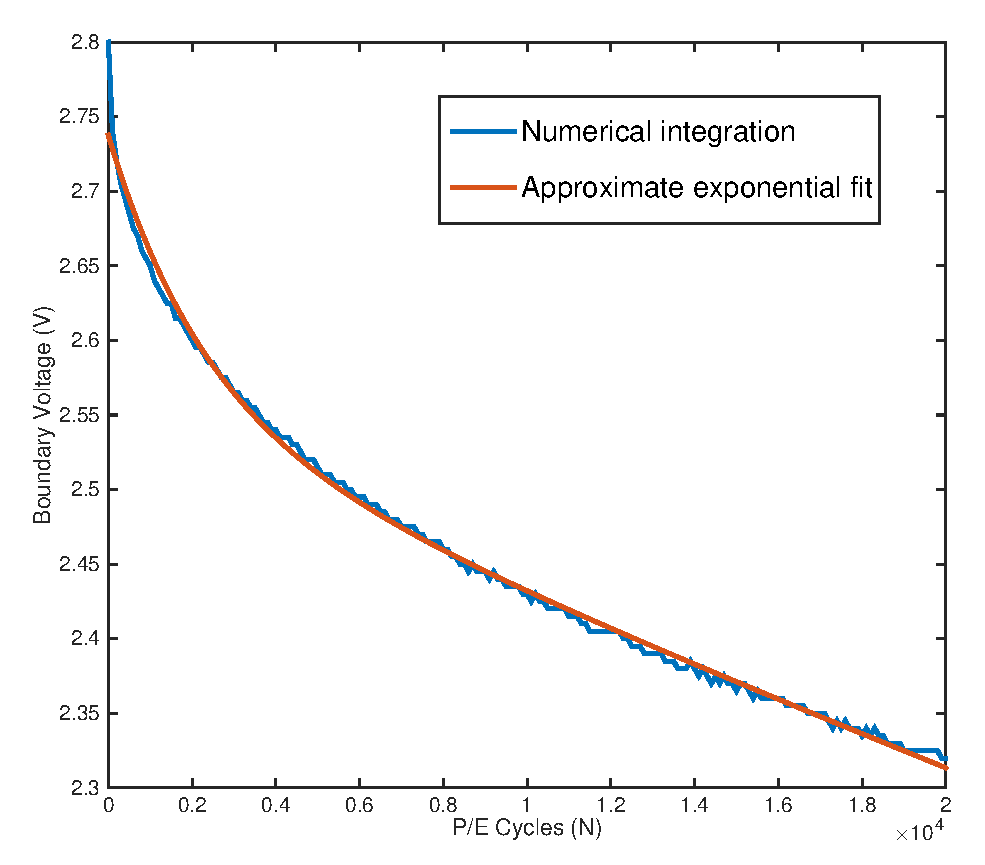
\includegraphics[scale=0.52]{variable_boundary_graph}
\caption{Results of numerical integration, showing ideal hard decision decoding boundary for given values of N}
\label{fig:hard_decision_variable_boundary}
\endminipage\hfill
\minipage{0.5\textwidth}
\centering
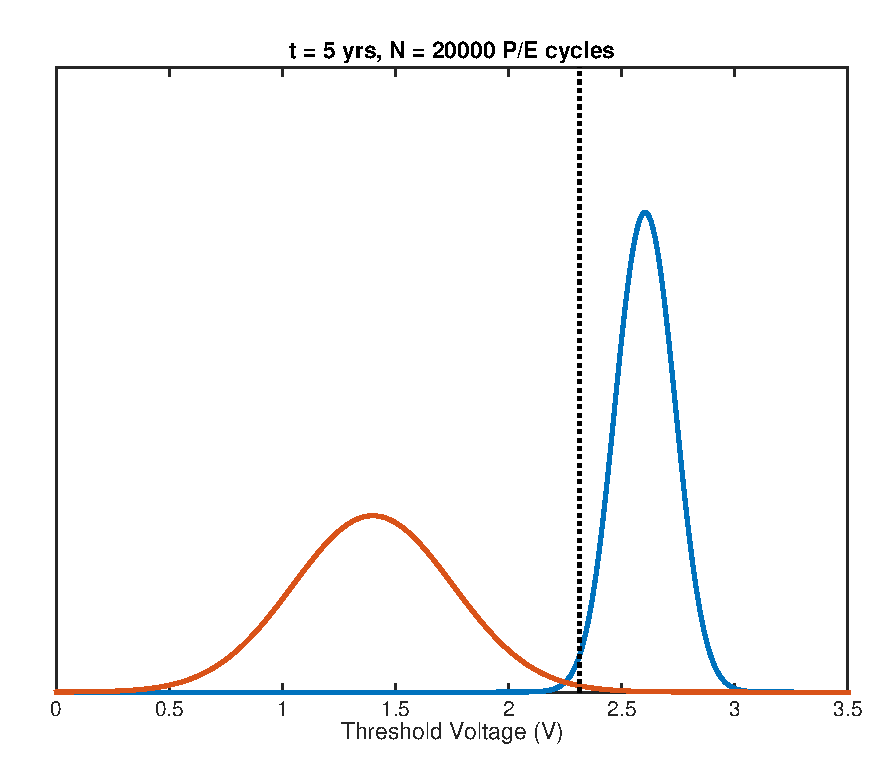
\includegraphics[scale=0.6]{variable_boundary_example}
\caption{Example showing both erased and programmed distributions and the decision boundary (dotted line) between them}
\label{fig:hard_decision_variable_example}
\endminipage
\end{figure}

Figure \ref{fig:hard_decision_variable_boundary} shows the results of the numerical integration, in order to obtain the optimal decision boundary for hard decision decoding. The boundary voltage, V, is the same as $x$ for the analytic case. The results appear slightly jagged since the data was taken from histograms of each distribution, which themselves were created from random sampling. In order to make use of the data from the integration, in a closed form solution, a simple exponential fit was plotted over the results. 

Figure \ref{fig:hard_decision_variable_example} is an example of both the erased and programmed distributions for a specific P/E cycle number, $N=20,000$. The dotted black line shows the optimal decision boundary, taken from the approximate exponential fit in figure \ref{fig:hard_decision_variable_boundary} ($V \approx 2.31$).

\subsection{Soft decision decoding: Gaussian approximations \& non-Gaussian functions}
As shown previously, soft decision decoding makes use of additional 'soft' information in order to improve the decoding performance. The main premise with SDD is to introduce probabilities into the decoding process, harnessing the \textit{a priori} probabilities of the underlying distributions, in order to construct a probabilistic decoder.

Simply obtaining the exact threshold voltage of the memory cell is not sufficient to perform SDD. As with the AWGN model, some prior information (in that case the noise variance) is required in order to convert the received raw data into a likelihood value. Once a likelihood \textit{ratio} of the received data has been calculated, exactly the same Sum-Product algorithm can be used as before. The difficulty in the memory model case, is obtaining this likelihood ratio.

\begin{equation} \label{eq:llr_memory}
\mathcal{L}(c|y) \sim log_e \left[ \dfrac{\text{\textit{``Probability density function of E(x)"}}}{\text{\textit{``Probability density function of P(x)"}}} \right]
\end{equation}

Equation \ref{eq:llr_memory}, which results from the earlier work in section \ref{section:LLR}, gives us the Log-Likelihood ratio that is required in order to perform soft decision decoding on the memory channel. It is clear that the necessary \textit{a priori} information in this case is the entire Probability Density Function for both the erased and programmed states. Once the PDF's are known, the voltage value for the cell can be inputted and the requisite LLR obtained.

As said previously, obtaining an exact solution for the density functions is non-trivial. This arises since, as explained in equation \ref{eq:additive_memory_noise_model}, we are adding both Gaussian and Laplacian noise onto a Uniform distribution in the case of the programmed state, and adding Laplacian noise to a Gaussian distribution in the case of the erased state.

To evaluate the overall probability density functions, given the individual PDF's of each noise source, requires using the convolution property:

\begin{equation} \label{eq:convProperty}
f_{1+2+...+N}(x) = (f_1 \ast f_2 \ast .... \ast f_N)(x)
\end{equation}
That is, the probability density function resulting from the sum of independent random variables, is just the convolution of each random variable's own density function. In terms of the memory model, this means the overall density function representing the programmed state is the 3-way convolution of a Gaussian, Laplacian and Uniform distribution. For the erased state, it is the convolution between a Gaussian and Laplacian. 

Performing such a convolution analytically, whilst possible, results in a function with a large number of terms. For example, the resultant PDF of the programmed state contains 6 exponential and 6 error ($\erf$) functions. Whilst using the full density function within the Log-Likelihood ratio gives the overall best performance, there may be ways to achieve similar performance by using a simpler approximation. In terms of the simulation, a simplified approximation would be able to run quicker in MATLAB, whilst in a real device, might be easier to implement. 

\subsubsection{Full convolution: Retention Noise + RTN} \label{section:fullFunc}
The full convolution of the initial Uniform distribution with the retention noise and RTN density function, the result of which was obtained from [Hachem ref], is shown below:
\begin{dmath}[label={eq:full_func}]
f_{prog}(\Delta V_{T}=x) = \frac{1}{4\Delta V_{pp}}e^{\frac{^{\sigma_{r}^{2}}}{2\lambda^{2}}}\left[e^{-\frac{x-Vp-\Delta V_{pp}-\mu_{r}}{\lambda}}\mathbf{\cdot erfc}\left(\frac{\sigma_{r}}{\sqrt{2}\lambda}-\frac{x-Vp-\Delta V_{pp}-\mu_{r}}{\sqrt{2}\sigma_{r}}\right)-e^{\frac{x-Vp-\Delta V_{pp}-\mu_{r}}{\lambda}}\mathbf{\cdot erfc}\left(\frac{\sigma_{r}}{\sqrt{2}\lambda}+\frac{x-Vp-\Delta V_{pp}-\mu_{r}}{\sqrt{2}\sigma_{r}}\right)\right]- \frac{1}{4\Delta V_{pp}}e^{\frac{\sigma_{r}^{2}}{2\lambda^{2}}}\left[e^{-\frac{x-Vp-\mu_{r}}{\lambda}}\mathbf{\cdot erfc}\left(\frac{\sigma_{r}}{\sqrt{2}\lambda}-\frac{x-Vp-\mu_{r}}{\sqrt{2}\sigma_{r}}\right)-e^{\frac{x-Vp-\mu_{r}}{\lambda}}\mathbf{\cdot erfc}\left(\frac{\sigma_{r}}{\sqrt{2}\lambda}+\frac{x-Vp-\mu_{r}}{\sqrt{2}\sigma_{r}}\right)\right]+\frac{1}{2\Delta V_{pp}}\mathbf{\cdot erfc}\left(\frac{x-Vp-\Delta V_{pp}-\mu_{r}}{\sqrt{2}\sigma_{r}}\right)- \frac{1}{2\Delta V_{pp}}\mathbf{\cdot erfc}\left(\frac{x-Vp-\mu_{r}}{\sqrt{2}\sigma_{r}}\right)
\end{dmath}
Equation \ref{eq:full_func} is the probability density function of the cell threshold voltage $V_{T}$ for the programmed state. $Vp$ is the initial programmed voltage, $\Delta V_{pp}$ is the programming step voltage, $\mu_{r}$ and $\sigma_{r}$ are the retention noise parameters from equation \ref{eq:retention}, and $\lambda$ is the parameter describing the RTN.

\subsubsection{Full convolution: Retention Noise only}
The magnitude of the RTN generated is substantially smaller than the magnitude of the retention noise. It therefore seems reasonable to ignore the effect of the RTN and perform the convolution of just the uniform and Gaussian distributions for the programmed state.
Starting with the definitions of both the retention noise and initial programmed state PDF's:

\begin{equation}
\text{Retention Noise: } Y_{retention} \sim \mathcal{N}(\mu_r,\sigma_r) = \dfrac{1}{\sigma_r\sqrt{2\pi}} \exp\left\{{-\dfrac{(x-\mu_r)^2}{2\sigma_r^2}}\right\}
\end{equation}
\begin{equation}
\text{Initial State: } V_{p_0} \sim \mathcal{U}(a,b) = \begin{dcases}
    \dfrac{1}{b-a},& \text{ for } x \in [a,b]\\
    0,              & \text{otherwise}
\end{dcases}
\end{equation}
The convolution property from equation \ref{eq:convProperty} can now be used to obtain the overall PDF:
\begin{equation} \label{eq:conv1}
\begin{aligned}
V_{p_0}(x) \ast Y_{ret}(x) &= \int_{-\infty}^{\infty} V(\tau)Y(t-\tau)\,\mathrm{d}\tau \\
&= \dfrac{1}{b-a} \int_{a}^{b} \dfrac{1}{\sqrt{2\pi\sigma_r^2}} \exp\left\{{-\dfrac{(t-\tau-\mu_r)^2}{2\sigma_r^2}}\right\}\mathrm{d}\tau
\end{aligned}
\end{equation}
By comparing the necessary convolution in \ref{eq:conv1} to that of the Normal distribution's cumulative distribution function (equation \ref{eq:normcdf}), the convolution can now be calculated as in equation \ref{eq:conv2}:
\begin{equation} \label{eq:normcdf}
\Phi(x) = \dfrac{1}{\sqrt{2\pi}} \int_{-\infty}^x e^{-t^2/2} \, \mathrm{d}t
\end{equation}
\begin{equation} \label{eq:conv2}
V_{p_0}(x) \ast Y_{ret}(x) = \dfrac{1}{b-a}\left[ \Phi\left(\dfrac{(x-a)-\mu_r}{\sigma_r}\right) - \Phi\left(\dfrac{(x-b)-\mu_r}{\sigma_r}\right)\right]
\end{equation}
This result shows that by adding Gaussian noise to a Uniform distribution, you obtain the difference between two normal CDF's, scaled by the Uniform width.

\begin{figure}[h]
\centering
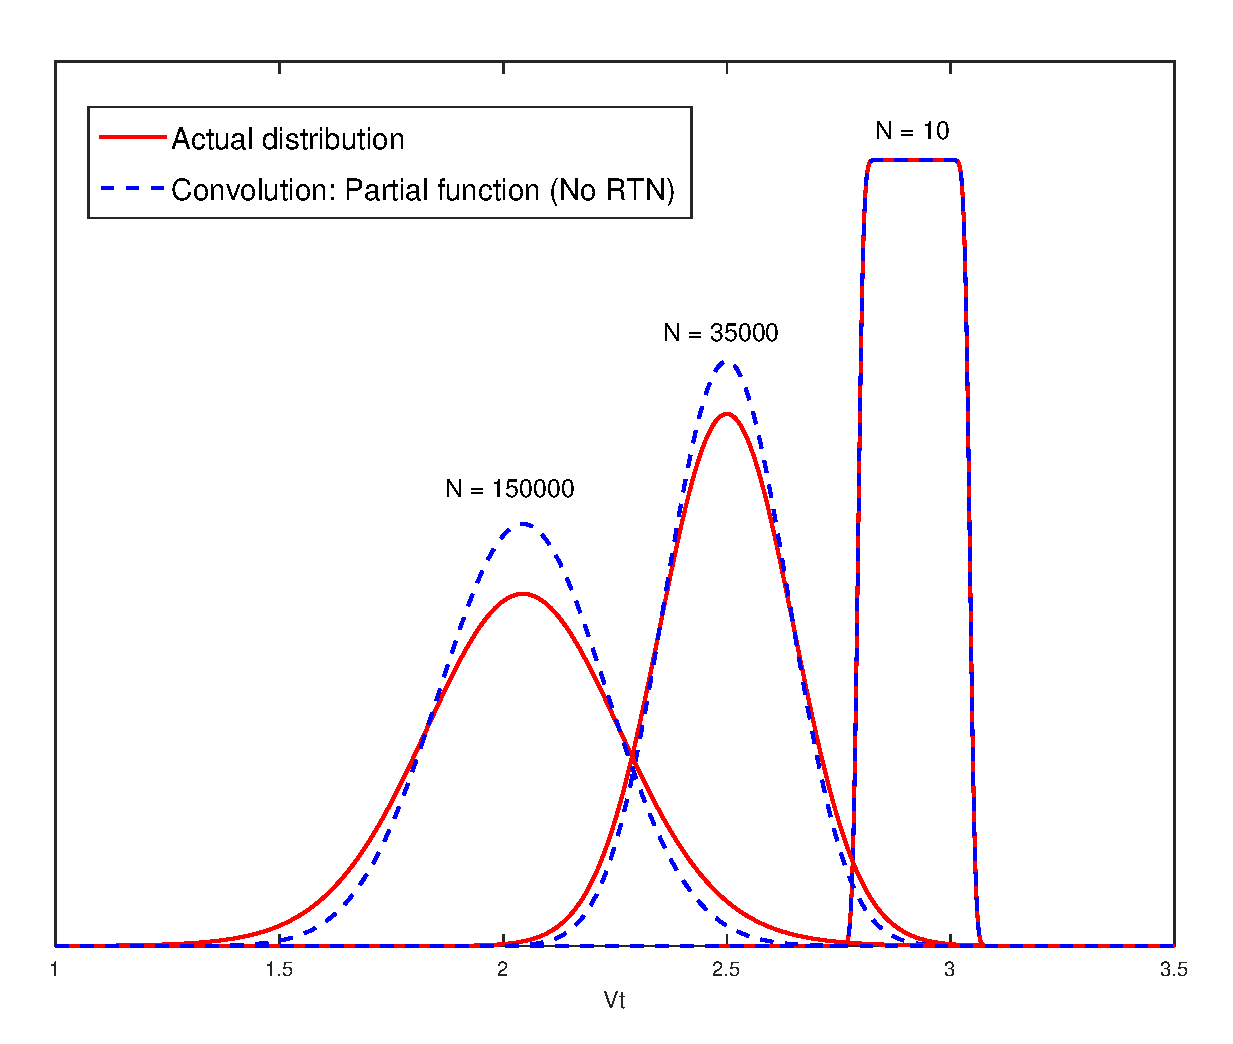
\includegraphics[scale=0.6]{retention_convolution}
\caption{Comparison of the distributions for different values of N}
\label{fig:retentionVsFull}
\end{figure}
Figure \ref{fig:retentionVsFull} shows that the convolution method, when excluding RTN, produces the correct shape of distribution for small N, but as N increases the difference between the distribution widens. This is because the RTN increases as N increases.

\subsubsection{Matched Gaussians}
Another approach to obtain the distribution of the threshold voltage, is to use a reasonable approximation of the function, rather than trying to obtain it directly. Using a simplified approximation also turns out to be faster [Around 5x faster when generating the LLR's in MATLAB compared to the full function in section \ref{section:fullFunc}].

An obvious choice would be to use a Gaussian. Whilst the distribution starts off as a Uniform distribution, adding noise causes it to quickly degrade into a gaussian-like shape. Since the memory noise model, as explained in equation \ref{eq:additive_memory_noise_model}, is addition of independent random variables, the mean and variance of each random variable can simply be added together to obtain the overall mean and variance of the distribution. These values can then be used to generate a 'Matched Gaussian', which will have the same mean and variance as the actual underlying function, but just with a slightly different shape. 
\begin{equation} \label{eq:matchedGaussians}
\begin{aligned}
\mu_p &= \mu_{p_0} + \mu_{rtn} + \mu_{retention} = \dfrac{2 V_p + \Delta V_{pp}}{2} + 0 +\mu_r \\
\sigma_p^2 &= \sigma^2_{p_0} + \sigma^2_{rtn} + \sigma^2_{retention} = \dfrac{\Delta V_{pp}^2}{12} + 2\lambda^2 + \sigma^2_{r}
\end{aligned}
\end{equation}
Thus, the equations in \ref{eq:matchedGaussians} show that the overall mean is just the mean of the uniform distribution plus the mean of the retention noise $\mu_r$, since the RTN distribution has a mean of zero. The variance is just the sum of the Uniform, Laplacian and Gaussian noise variances.
\begin{figure}[ht]
\centering
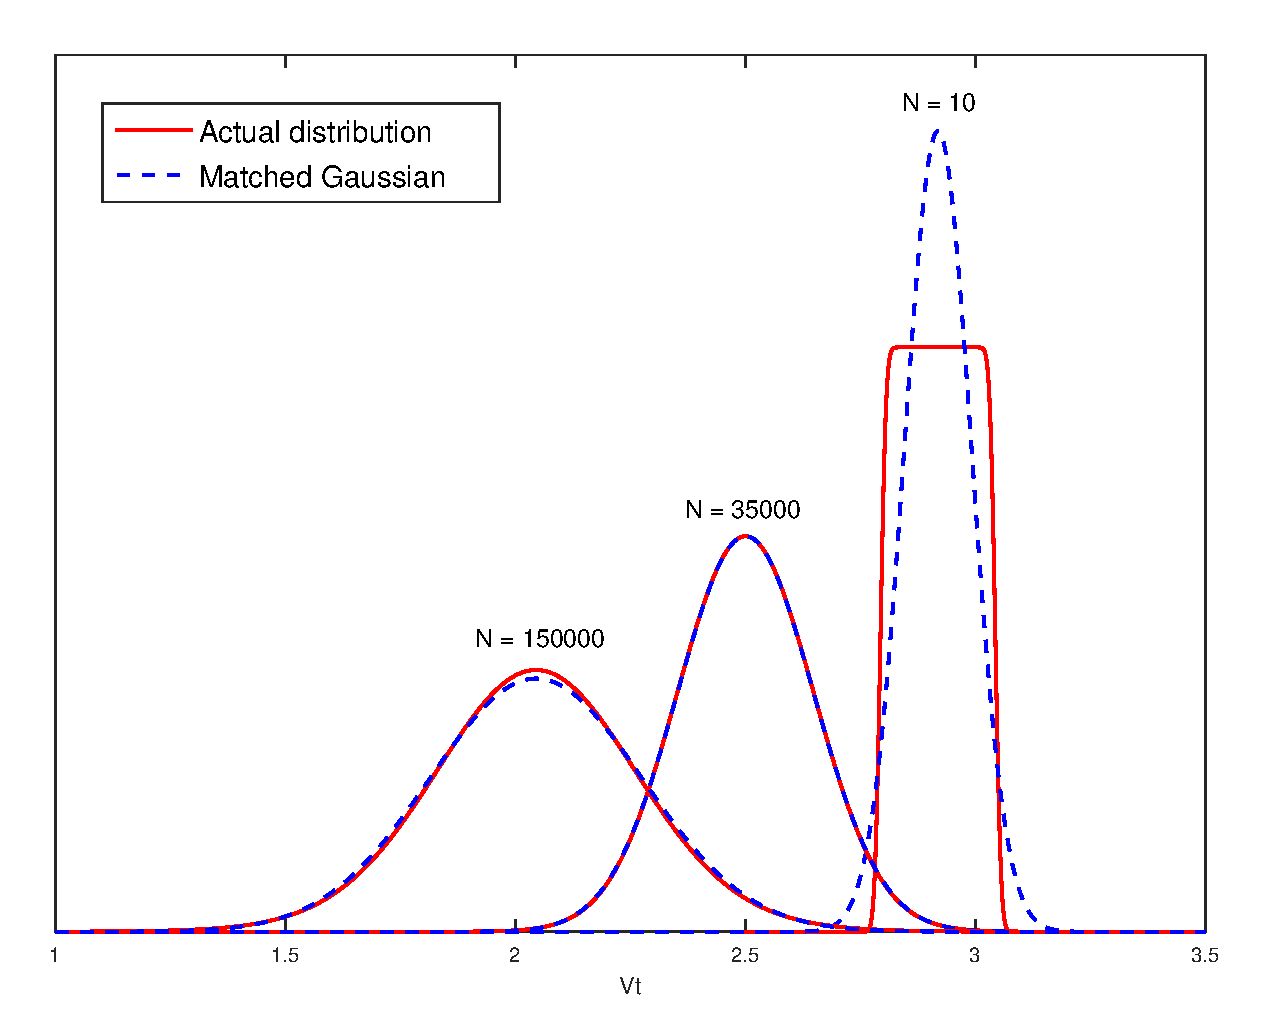
\includegraphics[scale=0.6]{matched_gaussian}
\caption{Comparison of the distributions for different values of N}
\label{fig:MMGaussianVsFull}
\end{figure}

Figure \ref{fig:MMGaussianVsFull} shows that using an approximation of the actual distribution can give, at least by inspection, very close results. Whilst the shape of the uniform distribution for small values of N is not successfully captured, for larger values of N the distributions appear to be a close match. 

\section{The memory channel: Simulation \& Results}
\subsection{Simulation Model}
The process for simulating the error correcting performance of the flash memory model is similar to the AWGN channel model that was used earlier. For the memory channel, a block of random binary data was generated, encoded to form an LDPC codeword, mapped to a cell threshold voltage, subject to some form of noise, detected and then finally decoded by the Belief Propagation algorithm to obtain the output data. By performing repeated trials of this process (Monte-Carlo simulation), for any given value of N, we can count the total number of bit errors over all simulated blocks, and obtain a bit-error rate (BER). 

\begin{figure}[h]
\centering
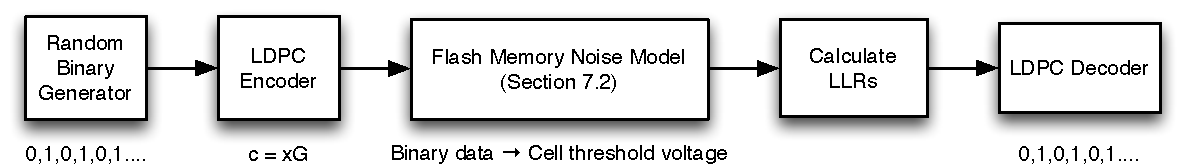
\includegraphics[scale=0.85]{memory_channel_model}
\caption{Memory simulation model}
\label{fig:mem_simulation_model}
\end{figure}

This simulation model is shown in figure \ref{fig:mem_simulation_model}. The 'Memory Noise Model' block encapsulates the entire process described in section \ref{section:memory_channel_model}, which includes mapping the input data to a cell threshold voltage, and then applying noise to that voltage, remembering that binary 1's and 0's are handled differently.

In this particular model, there are 2 independent variables that can be chosen: 'N', the number of program/erase cycles that the cell has undergone, and 't', the time in seconds that the data has been stored in that cell (the retention time). In addition, there are a number of initial conditions, which don't vary during the simulation. For the remainder of this project, 't' was fixed to 5 years, meaning that we are simulating the data written to the memory cell as having been stored there for 5 years. In initial testing, the variation of 't' had a substantially smaller effect on the overall bit-error rate of the system than varying 'N', and for simplicity that value was fixed. This is shown in figure \ref{fig:retention_time_graph}, where the uncoded (variable boundary hard decision method) bit-error rate of the memory cell is shown, and using a fixed 't' of 5 years has close results to using a 't' that varies as 'N' increases $(t = N/5000)$. Using a fixed value for 't' gives us a 'worst case scenario' of data undergoing a long retention time, even if this is unlikely in an actual scenario.
\begin{figure}[ht]
\centering
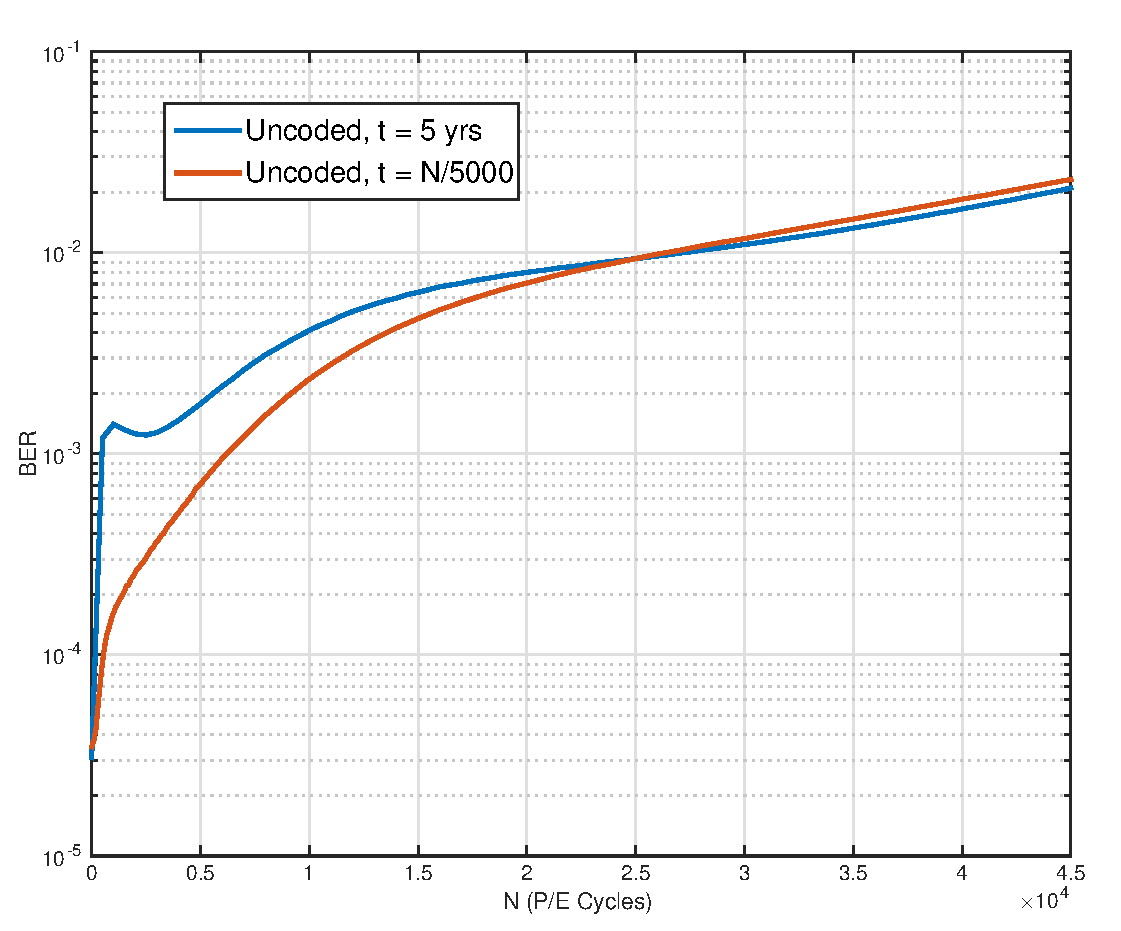
\includegraphics[scale=0.45]{retention_time_graph}
\caption{Comparing the effect of fixed t against using a variable t dependent on N}
\label{fig:retention_time_graph}
\end{figure}

\subsection{Simulation Results}
\begin{figure}[ht]
\centering
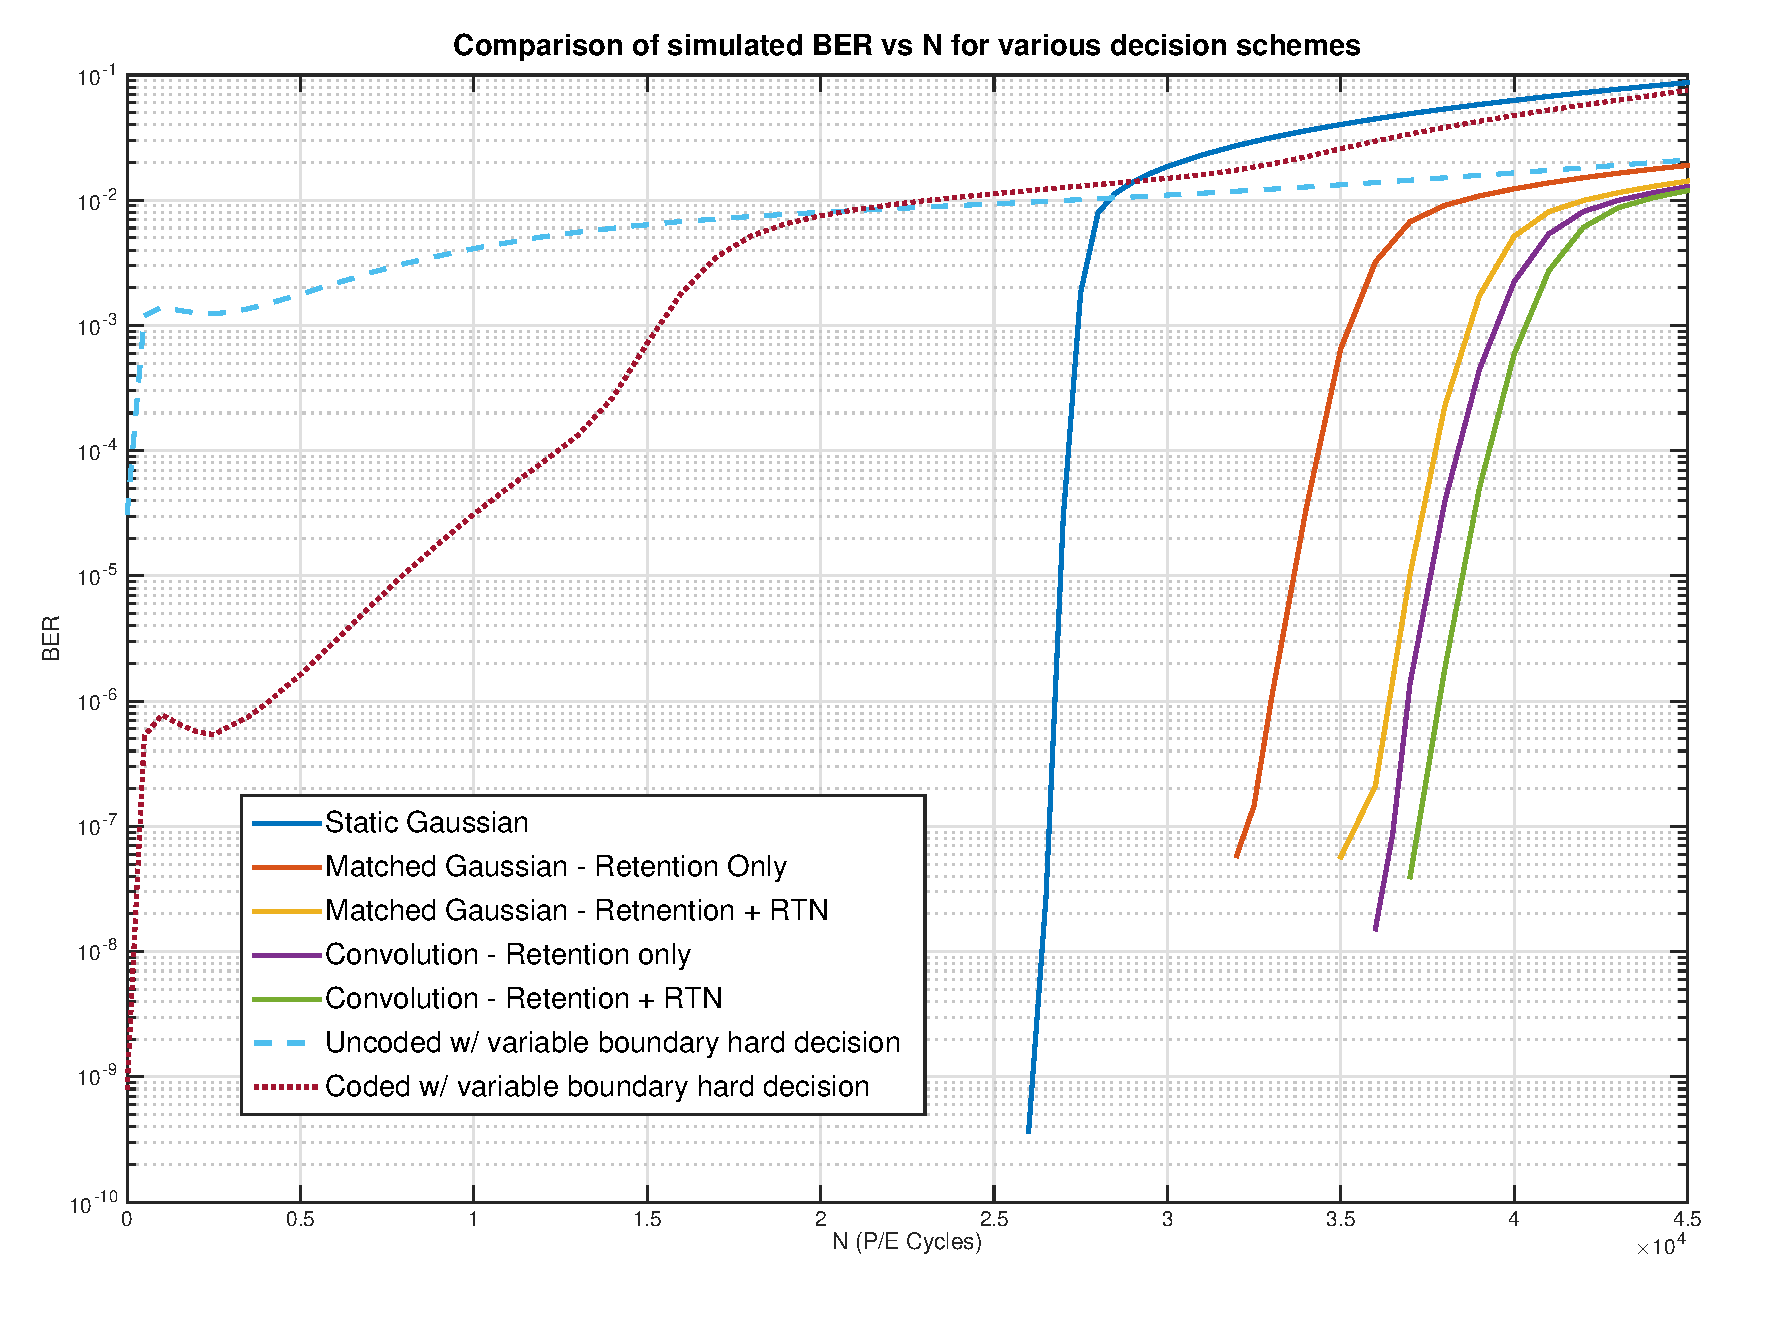
\includegraphics[scale=0.52]{codedBER_NCycles}
\caption{Graph of bit-error rate vs N for different decoding and LLR schemes}
\label{fig:memory_results_graph}
\end{figure}
\begin{figure}[ht]
\centering
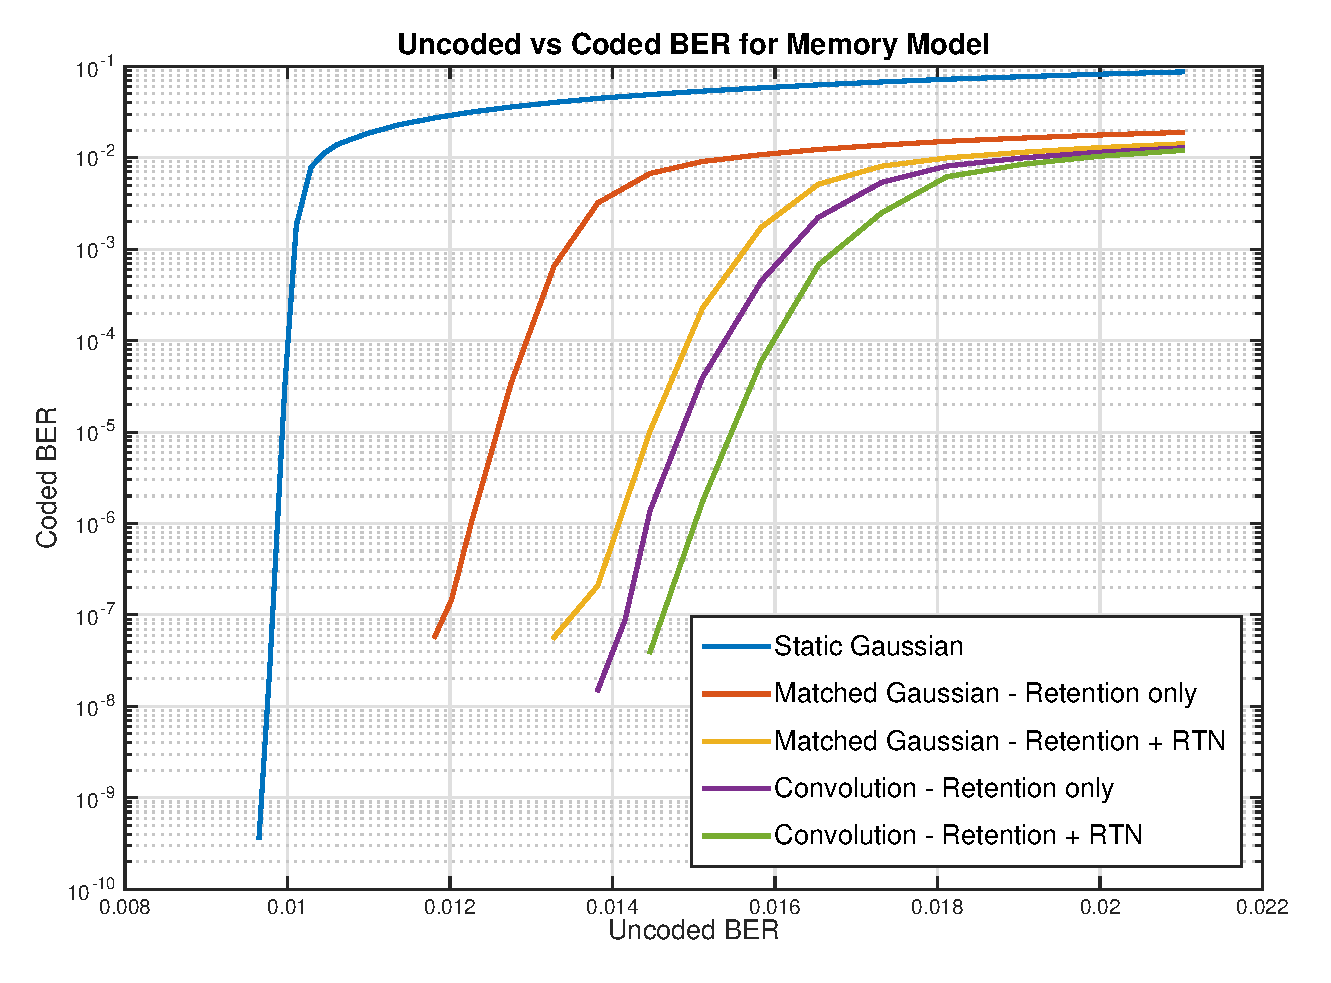
\includegraphics[scale=0.66]{cber_uber_memory}
\caption{Graph of uncoded vs coded bit-error rate for soft-decision cases}
\label{fig:memory_results_graph2}
\end{figure}

Monte-Carlo simulations were run on a remote cluster computer for each of the different decoding schemes explained in section \ref{section:memoryDecoding}. The results are shown in both figures \ref{fig:memory_results_graph} and \ref{fig:memory_results_graph2}.

Figure \ref{fig:memory_results_graph} shows the bit-error rate against a given 'N', the number of cell program/erase cycles. The solid lines all represent soft-decision decoding, each using a different approach when forming the LLR that is fed to the decoder. The 'Static Gaussian', whilst not explicitly declared earlier, uses a Gaussian centered about $V_{p_0}$, the initial programmed voltage. It is static since it doesn't move as N increases. This was the first attempt at performing soft-decision decoding for the system, and is essentially similar to the method of obtaining the LLR's for the AWGN channel (2 static Gaussian distributions).

The two matched Gaussians, one including the Random Telegraph Noise and one without, are the next best performing curves. It is clear that by adding the variance of the RTN to the Gaussian, it substantially improves performance of the decoder. However, the two functions obtained through the convolution of the various PDF's have the best overall performance. The green line, which is effectively making use of the exact underlying function in order to generate the LLR's, is therefore the upper bound on the performance of this system. 

Finally, the dotted line shows the performance of hard decision decoding. It is substantially worse performing than any of the soft decision methods, and only improves error performance against the uncoded case (the blue dashed line) by a relatively small margin, and only up to 20,000 cycles. Beyond this point, introducing error correction actually worsens the error performance of the system. 

Figure \ref{fig:memory_results_graph2} displays the same set of results for the soft decision schemes, but in a different format. The Coded vs Uncoded graph is a standard method used in industry to compare relative performance of error correction schemes. Essentially, given an uncoded system's bit error rate , it is possible to determine what the BER would be if an error correcting scheme is used. The uncoded BER in this case is taken from the hard decision, variable boundary method (the blue dashed line in the previous graph).

This particular graph construction is useful in comparing different systems, since it does not depend on the exact type of noise used. Instead, it allows us to easily compare what the error rate of the memory cell would be given a specific input error rate and coding scheme. For example, if the target bit error rate at the output of the system is to be $10^{-6}$, then an error rate of around $1\%$ in the memory cell is acceptable if using the Static Gaussian model. However, using the full PDF of the underlying noise in the decoder, an error rate of around $1.5\%$ is acceptable. Whilst this seems only a very small gain, by looking at figure \ref{fig:memory_results_graph} again, it actually results in the cell being able to endure an additional 10,000 cycles.

\section{Conclusions}
Placeholder

\phantomsection
\addcontentsline{toc}{section}{Appendix A: Random Number Generation}
\section*{Appendix A: Random Number Generation}
When performing any sort of Monte Carlo simulation, and particularly if running the same program in parallel across multiple computers, it is important to ensure that the random numbers being generated are as random as possible. Even more crucially, there must be no dependence between the parallel task's random numbers if we are to combine result sets.

MATLAB, like many other software packages, cannot generate truly random numbers. Instead, it uses a pseudo-random number generator, such as the Mersenne Twister algorithm. This is just a function that produces numbers which, for most purposes, are considered to be pseudo-random and pseudo-independent. That is, if you generate numbers from this algorithm, they will appear to be random samples from a uniform distribution. 

However, the Mersenne Twister algorithm actually has a finite period. After generating $2^{19937}$ random numbers, the output begins to repeat itself. More importantly, every time MATLAB starts, the random generator is reset to the same position. This means if you try to generate a large set of random numbers in MATLAB, you will always get exactly the same numbers. Effectively, MATLAB uses the same \textit{seed} to the random number generator on every start-up. This is meant to be useful for debugging purposes, however when running simulations in parallel, it causes all the result to no longer be independent. This means you cannot combine results made in parallel, since the output from each parallel stream will actually be identical.

The solution is to ensure that every task executed in parallel has a random seed fed into the random number generator. Effectively, the seed is used as the starting position for the Twister algorithm. If the seed is a truly random number, then each random generator should start in a different position. Any two random generators might start with billions of positions between them, or possibly right next to each other. But the chances of an identical start position are negligible.

\begin{lstlisting}[float=ht,style=Matlab-editor,caption = {Seeding random generator},label=code:rng]
% Ensures truly random numbers for each process
% seed is now a random number that can be used to initialise rand
fid = fopen('/dev/random');
seed = fread(fid, 1, 'uint32');
RandStream.setDefaultStream(RandStream('mt19937ar','seed',seed));
\end{lstlisting}

The commands in codebox \ref{code:rng} were used to seed the random number generator every time a new MATLAB process was created. On UNIX machines, there is a system random number source \mbox{`/dev/random'}, which ``gathers environmental noise from device drivers and other sources into an entropy pool [and] from this entropy pool random numbers are created." The numbers generated by this process originate from physical random processes such as hardware noise, and so it is assumed that when calling the function on a different machine, a different random number will be generated every time. These random numbers are then used to seed the pseudo-random stream in MATLAB.

\phantomsection
\addcontentsline{toc}{section}{Appendix B: MATLAB code}
\section*{Appendix B: MATLAB code}

\printbibliography

\end{document}